\documentclass[12pt,a4paper]{report}
\usepackage[brazilian, english]{babel}
\usepackage[utf8]{inputenc}
\usepackage[T1]{fontenc}
\usepackage{amsmath,amsthm,amsfonts,amssymb,textcomp}
%\usepackage{latexsym}
\usepackage{graphicx}
\graphicspath{{figuras}}
\usepackage{subfigure}
\usepackage{float}
\usepackage{longtable}
\usepackage{color}
\usepackage{epstopdf}
\usepackage{pdflscape}
\usepackage[breaklinks=true]{hyperref}
\usepackage[comma,authoryear]{natbib}
\usepackage[nonumberlist]{glossaries}
\usepackage{arydshln}
\usepackage{footnote}
\usepackage{longtable}
\usepackage[small,bf,singlelinecheck=off]{caption}
\usepackage[left=3cm,right=2cm,top=3cm,bottom=2cm]{geometry}
%\usepackage[alf]{abntcite}

%%% newcommand %%%%%%%%%%%%%%%%%
\newcommand{\PE}{Perkin-Elmer }
\newcommand{\BC}{Boller \& Chivens }

\newcommand{\degr}{\ensuremath{^{\circ}}}%                    % degree symbol:  °
\newcommand{\arcmin}{\ensuremath{^{\prime}}}%                    % degree symbol:  °
\newcommand{\arcsec}{\ensuremath{^{\prime\prime}}}%                    % degree symbol:  °
\newcommand{\fs}{\mbox{\ensuremath{.\!\!^s}}}
\newcommand{\farcm}{\mbox{\ensuremath{.\mkern-4mu^\prime}}}%    % fractional arcminute symbol: 0.'0
\newcommand{\farcs}{\mbox{\ensuremath{.\!\!^{\prime\prime}}}}%  % fractional arcsecond symbol: 0.''0
\newcommand{\fdg}{\mbox{\ensuremath{.\!\!^\circ}}}%             % fractional degree symbol:     0.°0



%\makeglossaries

\makeatletter
\renewcommand\chapter{\thispagestyle{plain}
                \global\@topnum\z@
                \@afterindentfalse
                \secdef\@chapter\@schapter}
\makeatother


\makeatletter
\renewcommand{\@makechapterhead}[1]{%
\vspace*{50 pt}%
{\setlength{\parindent}{0pt} \raggedright \normalfont
\bfseries\Huge\thechapter.\ #1
\par\nobreak\vspace{40 pt}}}
\makeatother

%\newglossaryentry{Offset}{name={Offset}, description={Diferença entre a posição obtida pela redução da observação e a posição dada pela efeméride}}
\newglossaryentry{OPD}{name={OPD}, description={Observatório do Pico dos Dias - Brasópolis, MG}}
\newglossaryentry{LNA}{name={LNA}, description={Laboratório Nacional de Astrofísica - Itajubá, MG}}
\newglossaryentry{OHP}{name={OHP}, description={Observatoire Haute Provence - Saint-Michel-l'Observatoire, França}}
\newglossaryentry{RA}{name={RA}, description={Sigla para Ascensão Reta ($ \alpha $)}}
\newglossaryentry{DEC}{name={DEC}, description={Sigla para Declinação ($ \delta $)}}
\newglossaryentry{Anomalia Verdadeira}{name={Anomalia Verdadeira}, description={Ângulo formado entre o Periastro e a posição instantânea do objeto na órbita centrado no planeta e contada na direção do movimento orbital}}
\author{Altair Ramos Gomes Júnior}
\title{Astrometry of the Neptune-Triton System}
\begin{document}

\maketitle

\pagestyle{headings}

\section*{Introduction}

In this report I present the preliminary results of the astrometric reductions of the images from the Observatório do Pico dos Dias (OPD) in Brazil. The aim is to obtain precise positions for the Neptune - Triton system. The telescopes used was the \PE (160) with a diameter of 1.6m, the \BC (IAG) with a diameter of 0.6m, and the Zeiss telescope with a diameter of 0.6m.

The observations were carried out since 1992 when a CCD big enough was installed in the OPD. The planet and satellite have been constantly observed, and still are, by our group. There were many CCDs (IKON, IXON, CCD101, CCD106, ...) and many filters (V, R, I, No Filter, ...) utilized.

%\section*{Data}

In Table \ref{Tab:dados} it is summarized the final number of images for Neptune and Triton for the 3 telescopes. It is also shown the number of positions where Neptune and Triton were identified automatically in the same image.

\begin{table*}[h]
\centering
\caption{Number of positions by object by telescope}
\label{Tab:dados}
\begin{tabular}{|c|c|c|c|}
\hline 
Telescope & Neptune & Triton & Matches \\ 
\hline
160 & 610 & 1154 & 547 \\ 
\hline 
IAG & 2381 & 2659 & 1888 \\ 
\hline 
Zeiss & 258 & 345 & 222 \\ 
\hline 
Total & 3249 & 4158 & 2657 \\ 
\hline 
\end{tabular}
\\Number of positions identified of Neptune and Triton by telescope. In parentheses the number of nights where the observations are distributed. Matches: Number of positions where Neptune and Triton were identified automatically in the same image.
\end{table*}

There were a total of 9942 images from June 1992 to September 2015. Many of the oldest images had no coordinates in header or they were wrong. Sometimes the filter was missing. Many nights had two exposure sets. The first one with low exposure time so Neptune were not saturated, but there were few reference stars in the field. The second one with higher exposure time so Triton were brighter and had more reference stars the the previous exposure, but the image of Neptune were saturated.

Fig. 1 shows the distribution of positions identified for Neptune and Triton over the years.

\begin{figure}[h]
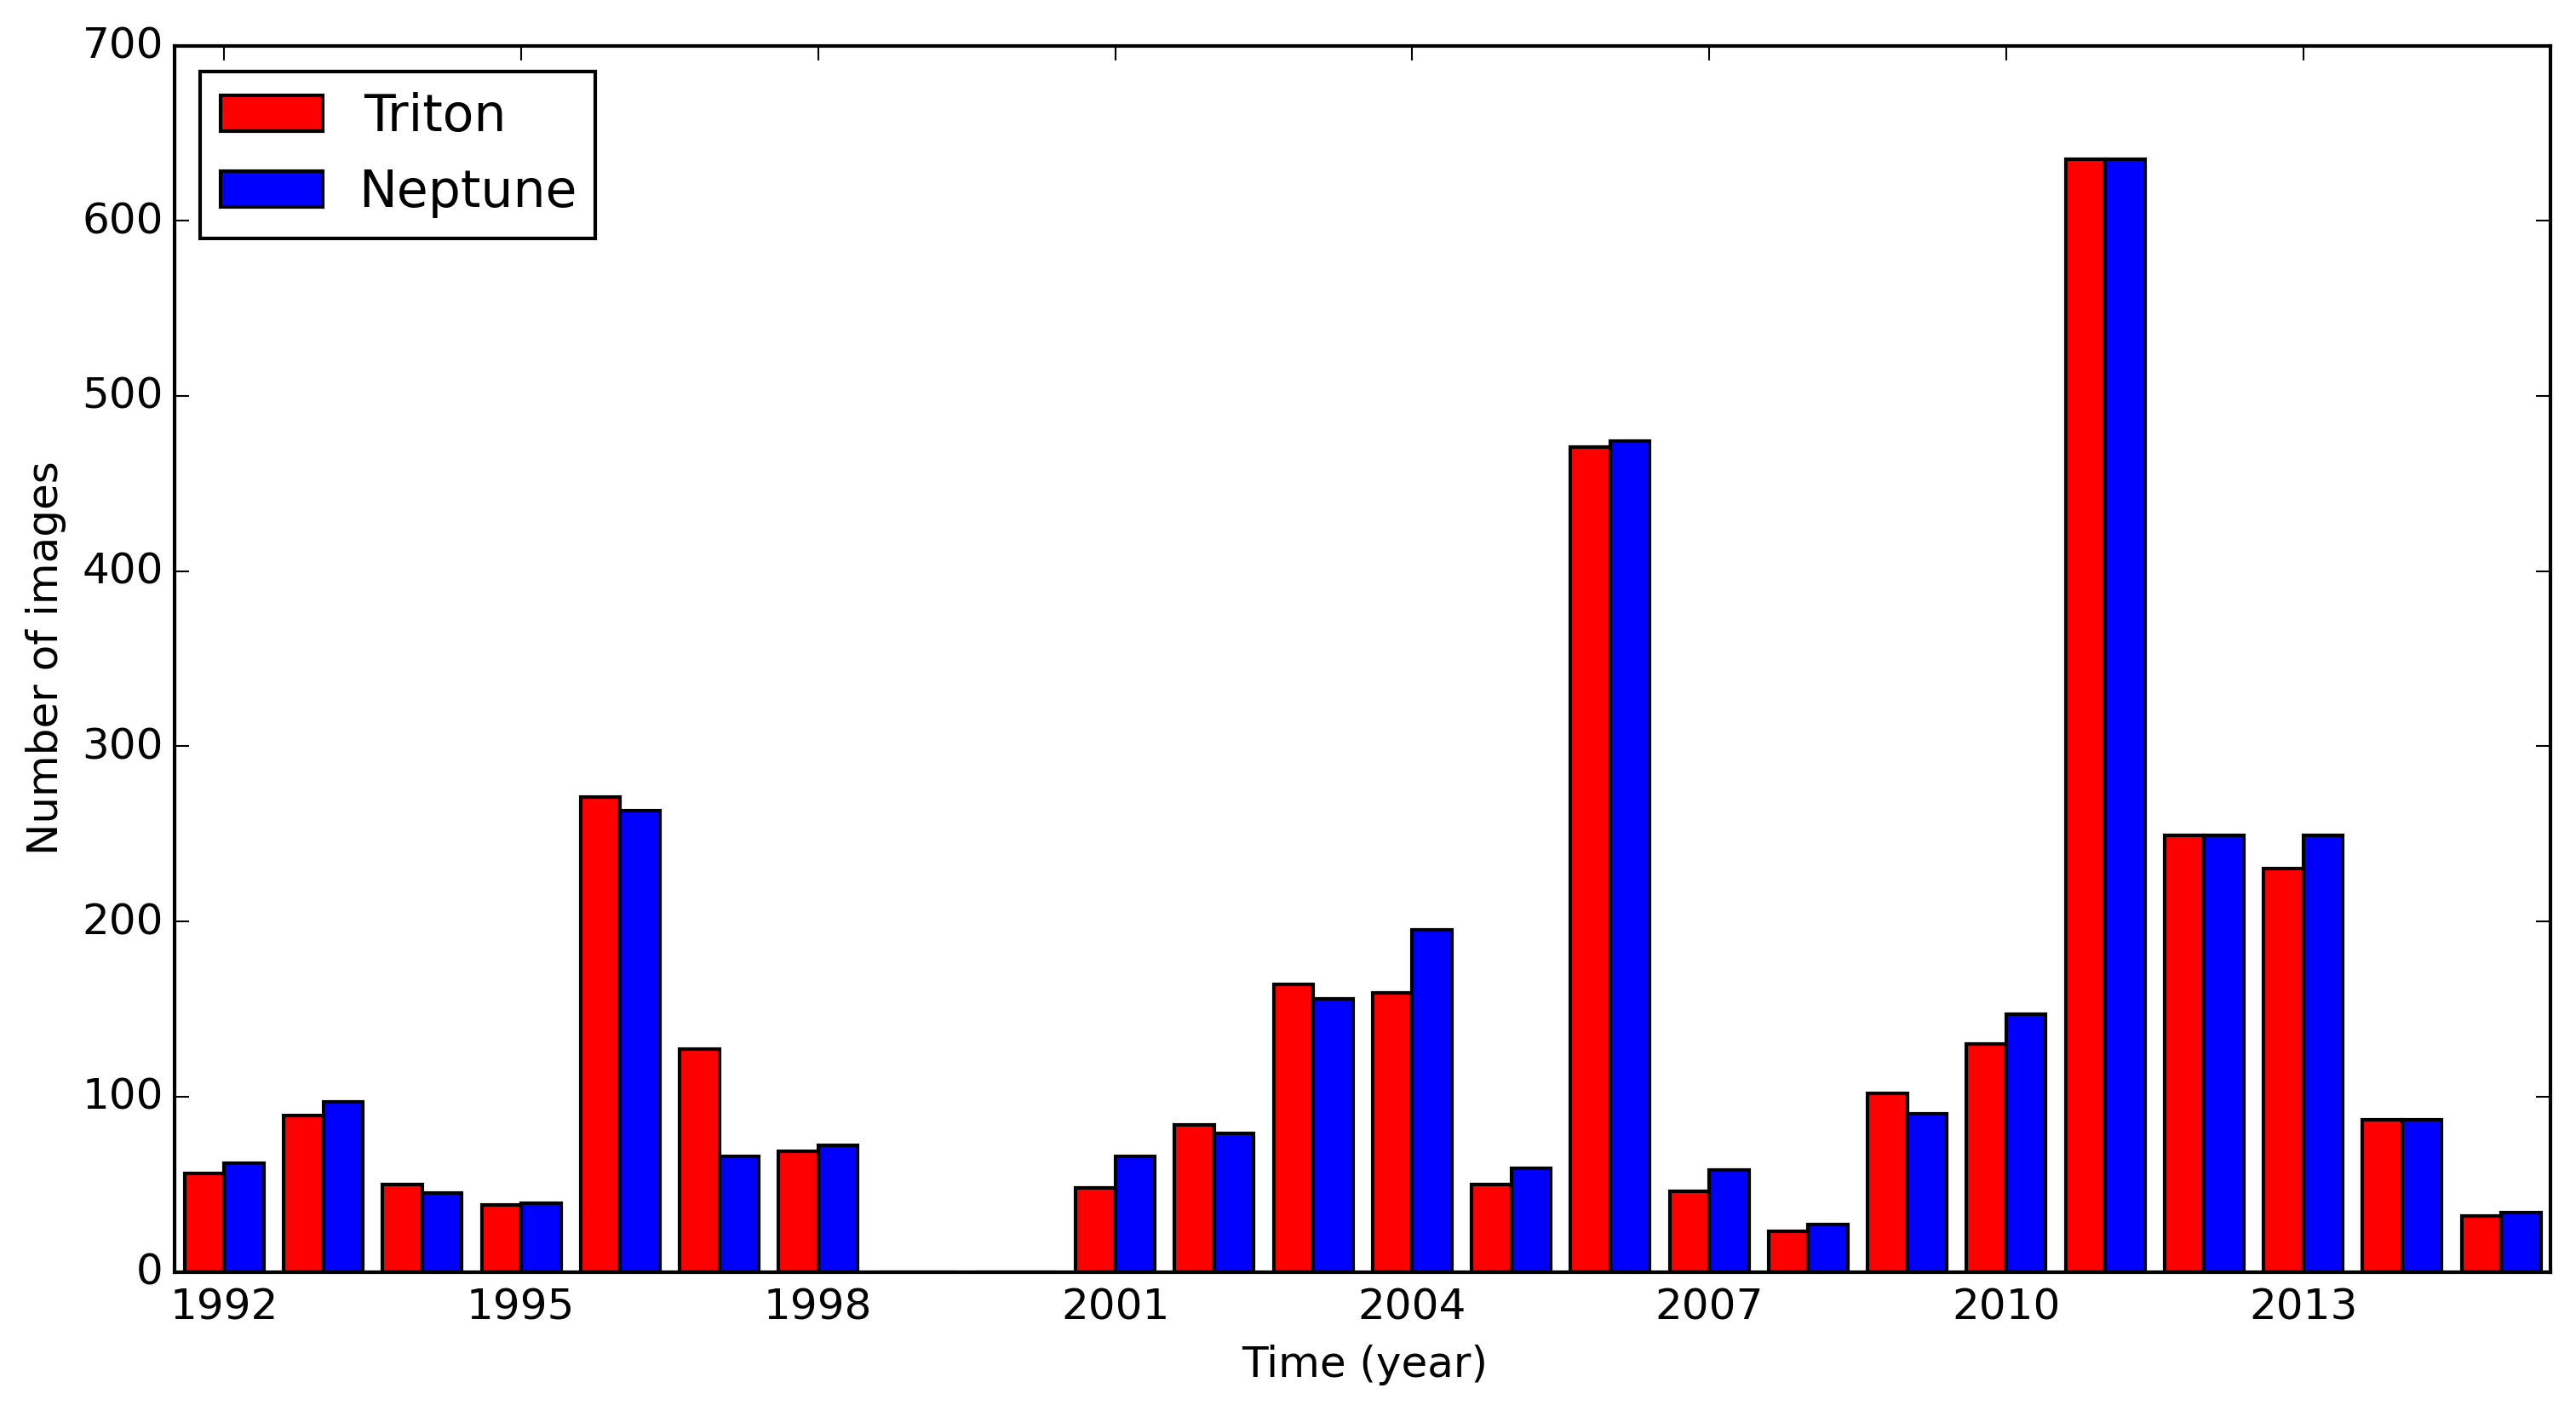
\includegraphics[width=16.0cm]{pos-distribution.png} 
\caption{Distribution of positions for Neptune and Triton by year}
\label{Fig:pos-dist}
\end{figure}


\section*{Reduction}

The images were reduced using PRAIA, developed by Marcelo Assafin. To avoid the missing or wrong coordinates I used the coordinates of the ephemeris as input. This way PRAIA could identify reference stars in the images. The reference catalogue used was UCAC4. The ephemeris used to identify Neptune and Triton in the images was DE430+NEP081. The positions where the image of Neptune were saturated was removed of the results.

We applied the digital coronagraphy technique to test if the scattered light of Neptune would influence in the Triton's photocenter. No influence was identified in the 1 mas range.

From the offsets in the sense "position minus ephemeris" identified I made statistics night by night to eliminate discrepant positions with a sigma-clip procedure where offsets (modulus) larger than 80 mas or 2-sigma discrepant from the mean offset were removed.

We also tested two other process of reduction in the nights with two different exposure sets. The first one is the uniform reduction where only stars presented in all fields were used to represent the reference system. The second one is the global reduction where all the stars presented in all fields are used within a unique least-square procedure to obtain the reference system. With this, four situations were considered.

\begin{enumerate}
\item The standard procedure of astrometric reduction.
\item The uniform reduction of the fields.
\item The global reduction over the identified stars in the procedure 1.
\item The global reduction over the identified stars in the procedure 2.
\end{enumerate}

For each situation we tested two sets of positions. The first one with the positions of Neptune and Triton within the same exposure set as explained above. The second one with the positions of Neptune in the smallest exposure set and the positions of Triton in the biggest exposure set (where Neptune were saturated).

For each night tested, we obtained the mean difference in the offsets of Triton-Neptune for the 4 situations and the 2 sets of positions. The dispersion of the 4 situations for the set where Neptune and Triton have the same exposure is in majority smaller than the set where they have different exposures.

Figs 2 e 4 show the offsets of Neptune and Triton, respectively, in RA e DEC for all the positions not eliminated in the previous procedure. Figs 3 e 5 show the mean offsets of each night and respective discrepancy (error bars).

Fig 6 shows the difference between the relative observed positions and the relative ephemeris positions of Triton and Neptune in the sense Triton - Neptune where they were identified in the same frame and not eliminated by the sigma-clip procedure.

Fig 7 shows the difference in the mean offsets night by night for all matched nights and not eliminated by the sigma-clip procedure in the sense Triton - Neptune. The dispersions (error bars) is the mean value of the dispersion in the night for each satellite.

%The large offsets found in 2002-2003 must be checked. It may be caused by few reference stars in the field or saturation.\\


We plan to do the following:
\begin{itemize}
\item Separate images by filter.
\item Study the effects of chromatic refraction in the offsets (difference of offsets Triton - Neptune). I already have nights separated with observations distributed over six hours during the night.
\item It may be required the use of a specific PSF for Neptune due to its large size.
\item Further refinements in the data may be needed as we further investigate these position sets.
\end{itemize}

Figures 8-10 summarizes the distribution of positions by filter obtained in the \PE , the \BC and the Zeiss telescopes, respectively.

%In Tables 2 and 3 it is shown the mean offsets in Right Ascension and Declination night by night for Neptune and Triton, respectively, observed in the \PE telescope. The dispersion of the positions (standard deviation), number of frames that was not eliminated by the sigma-clip procedure, the mean date of the night and the average number of reference stars by frame is also available in the tables. The respective mean offsets night by night for the \BC telescope is available in Tables 4 and 5. As for the previous telescopes, tables 6 and 7 summarizes the offsets obtained with the Zeiss telescope.

In Table 2 it is presented the mean errors in X and Y of the bidimensional Gaussian used to fit the PSF of the objects. %The average dispersion of the offsets in Tables 2-7 is also presented in the table.


\begin{figure}[h]
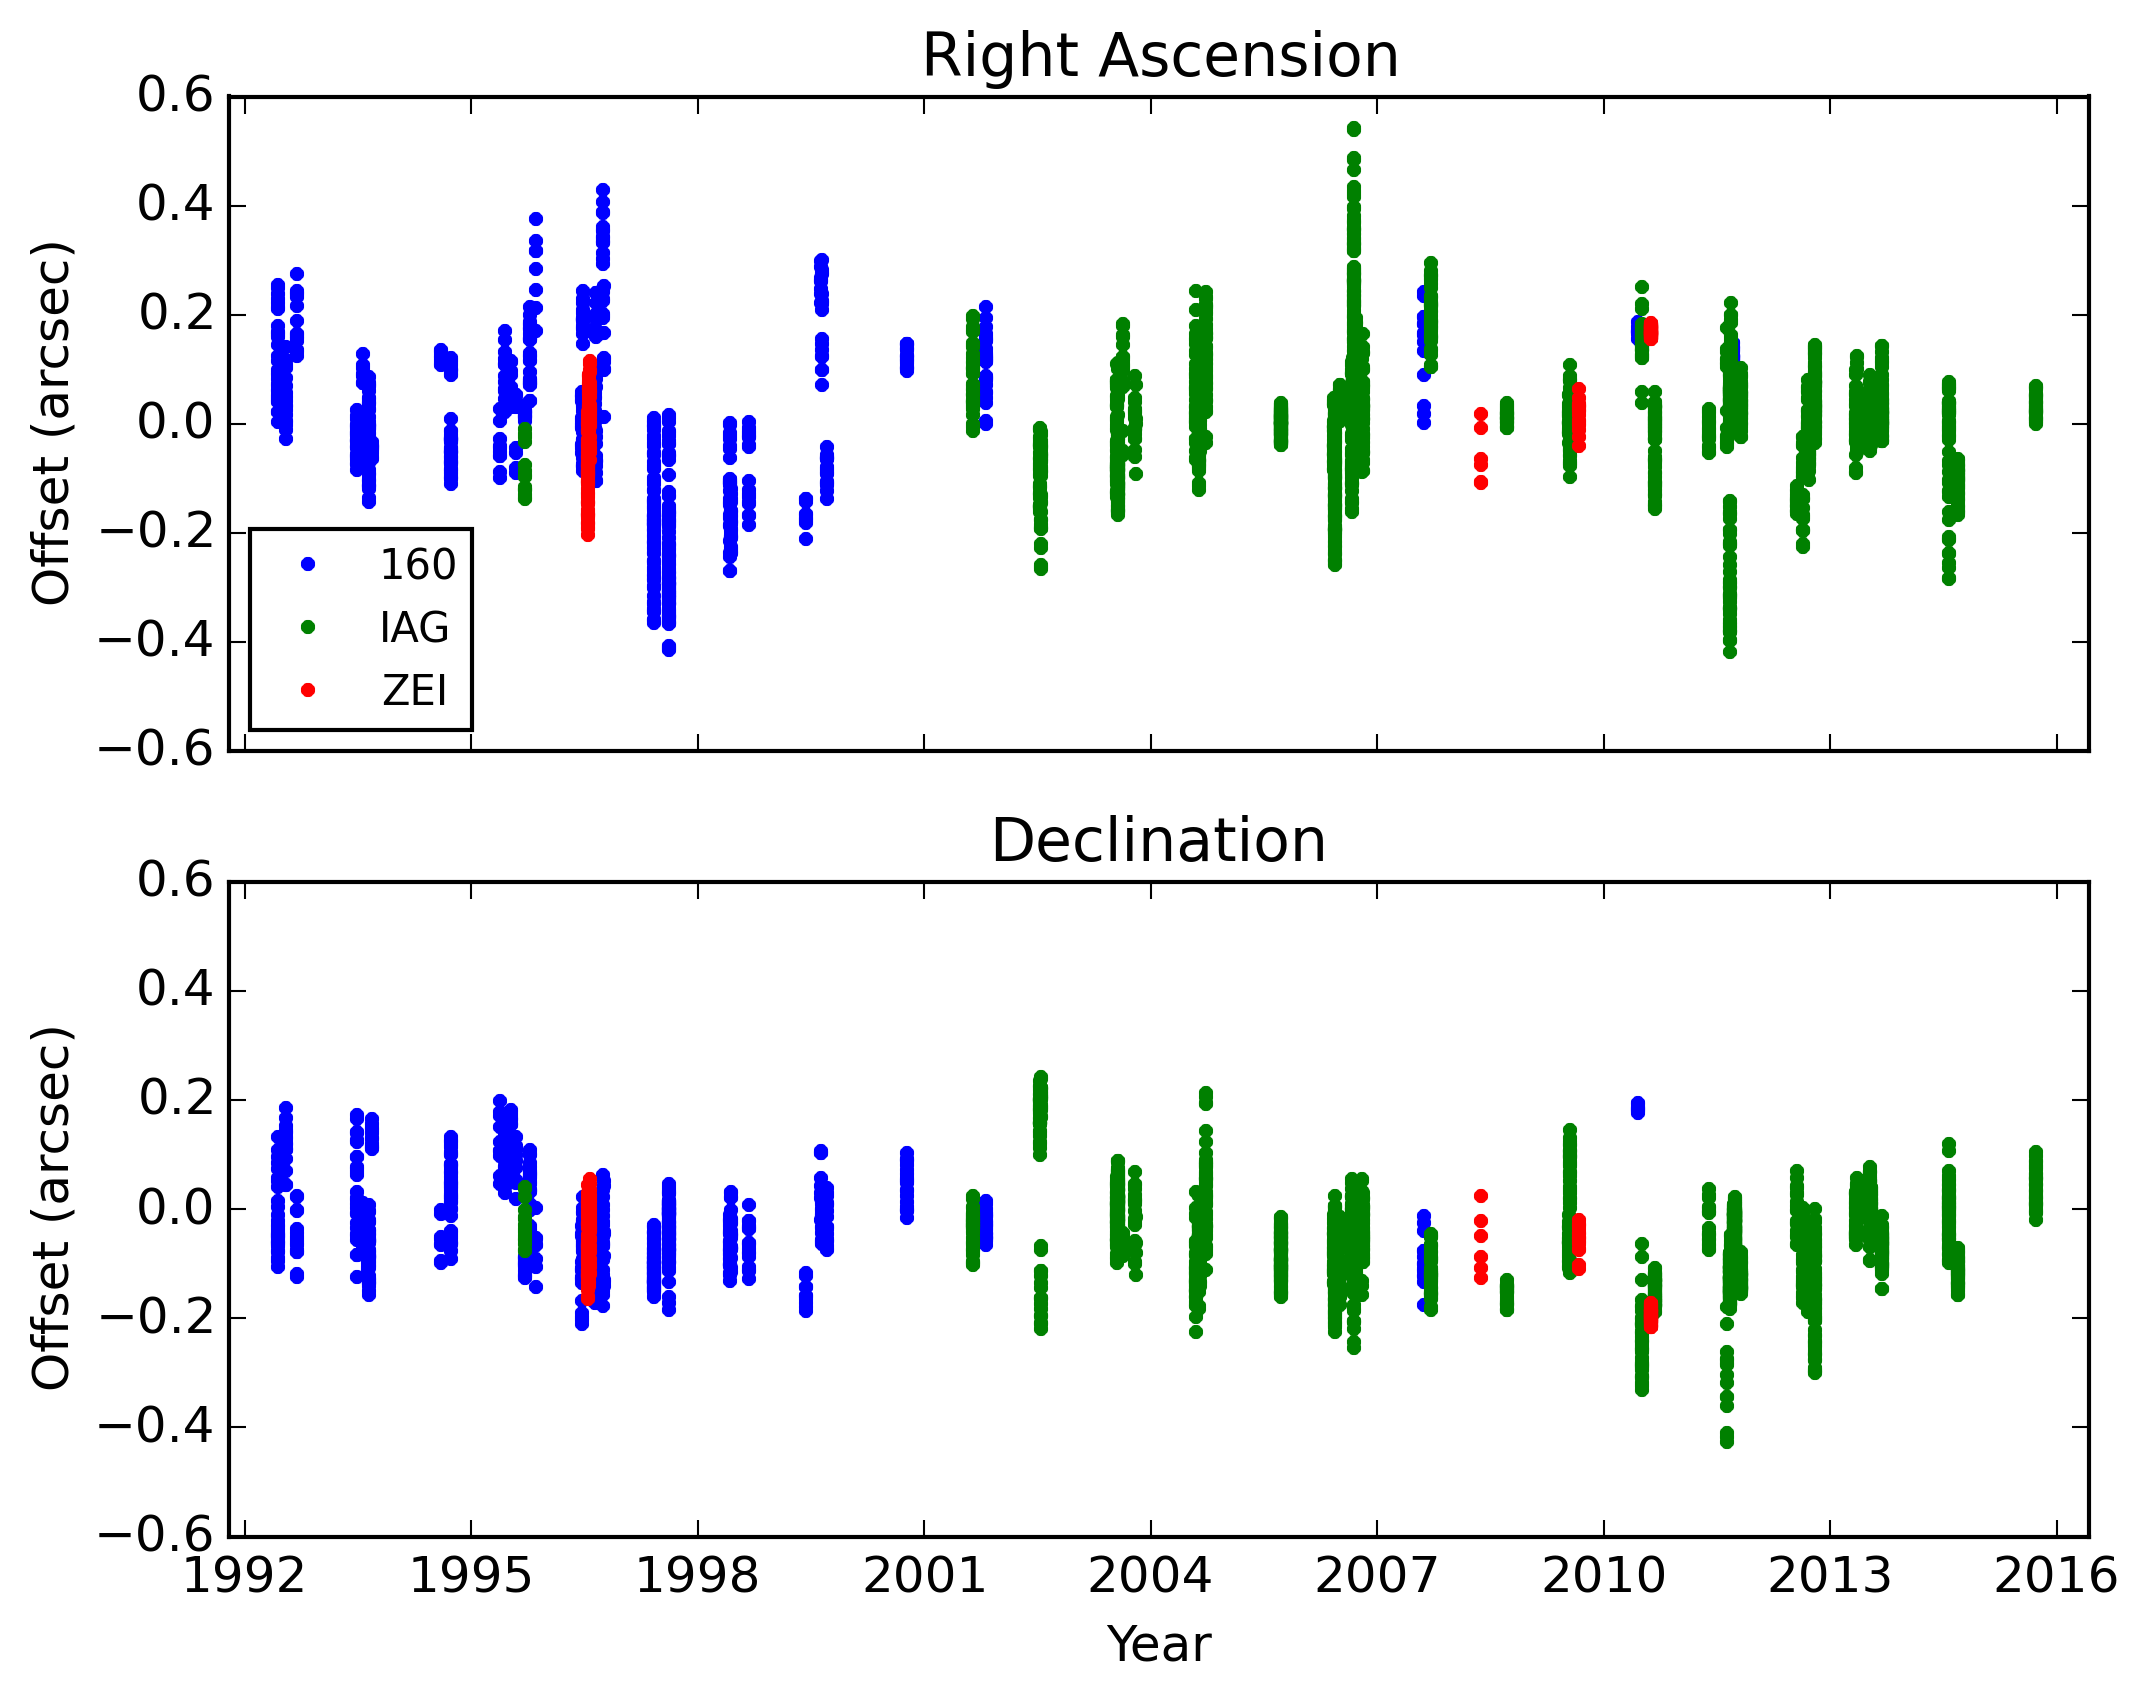
\includegraphics[width=16.0cm]{Netuno_all.png} 
\caption{Neptune - All Offsets}
\label{Fig:netuno-all}
\end{figure}
\begin{figure}
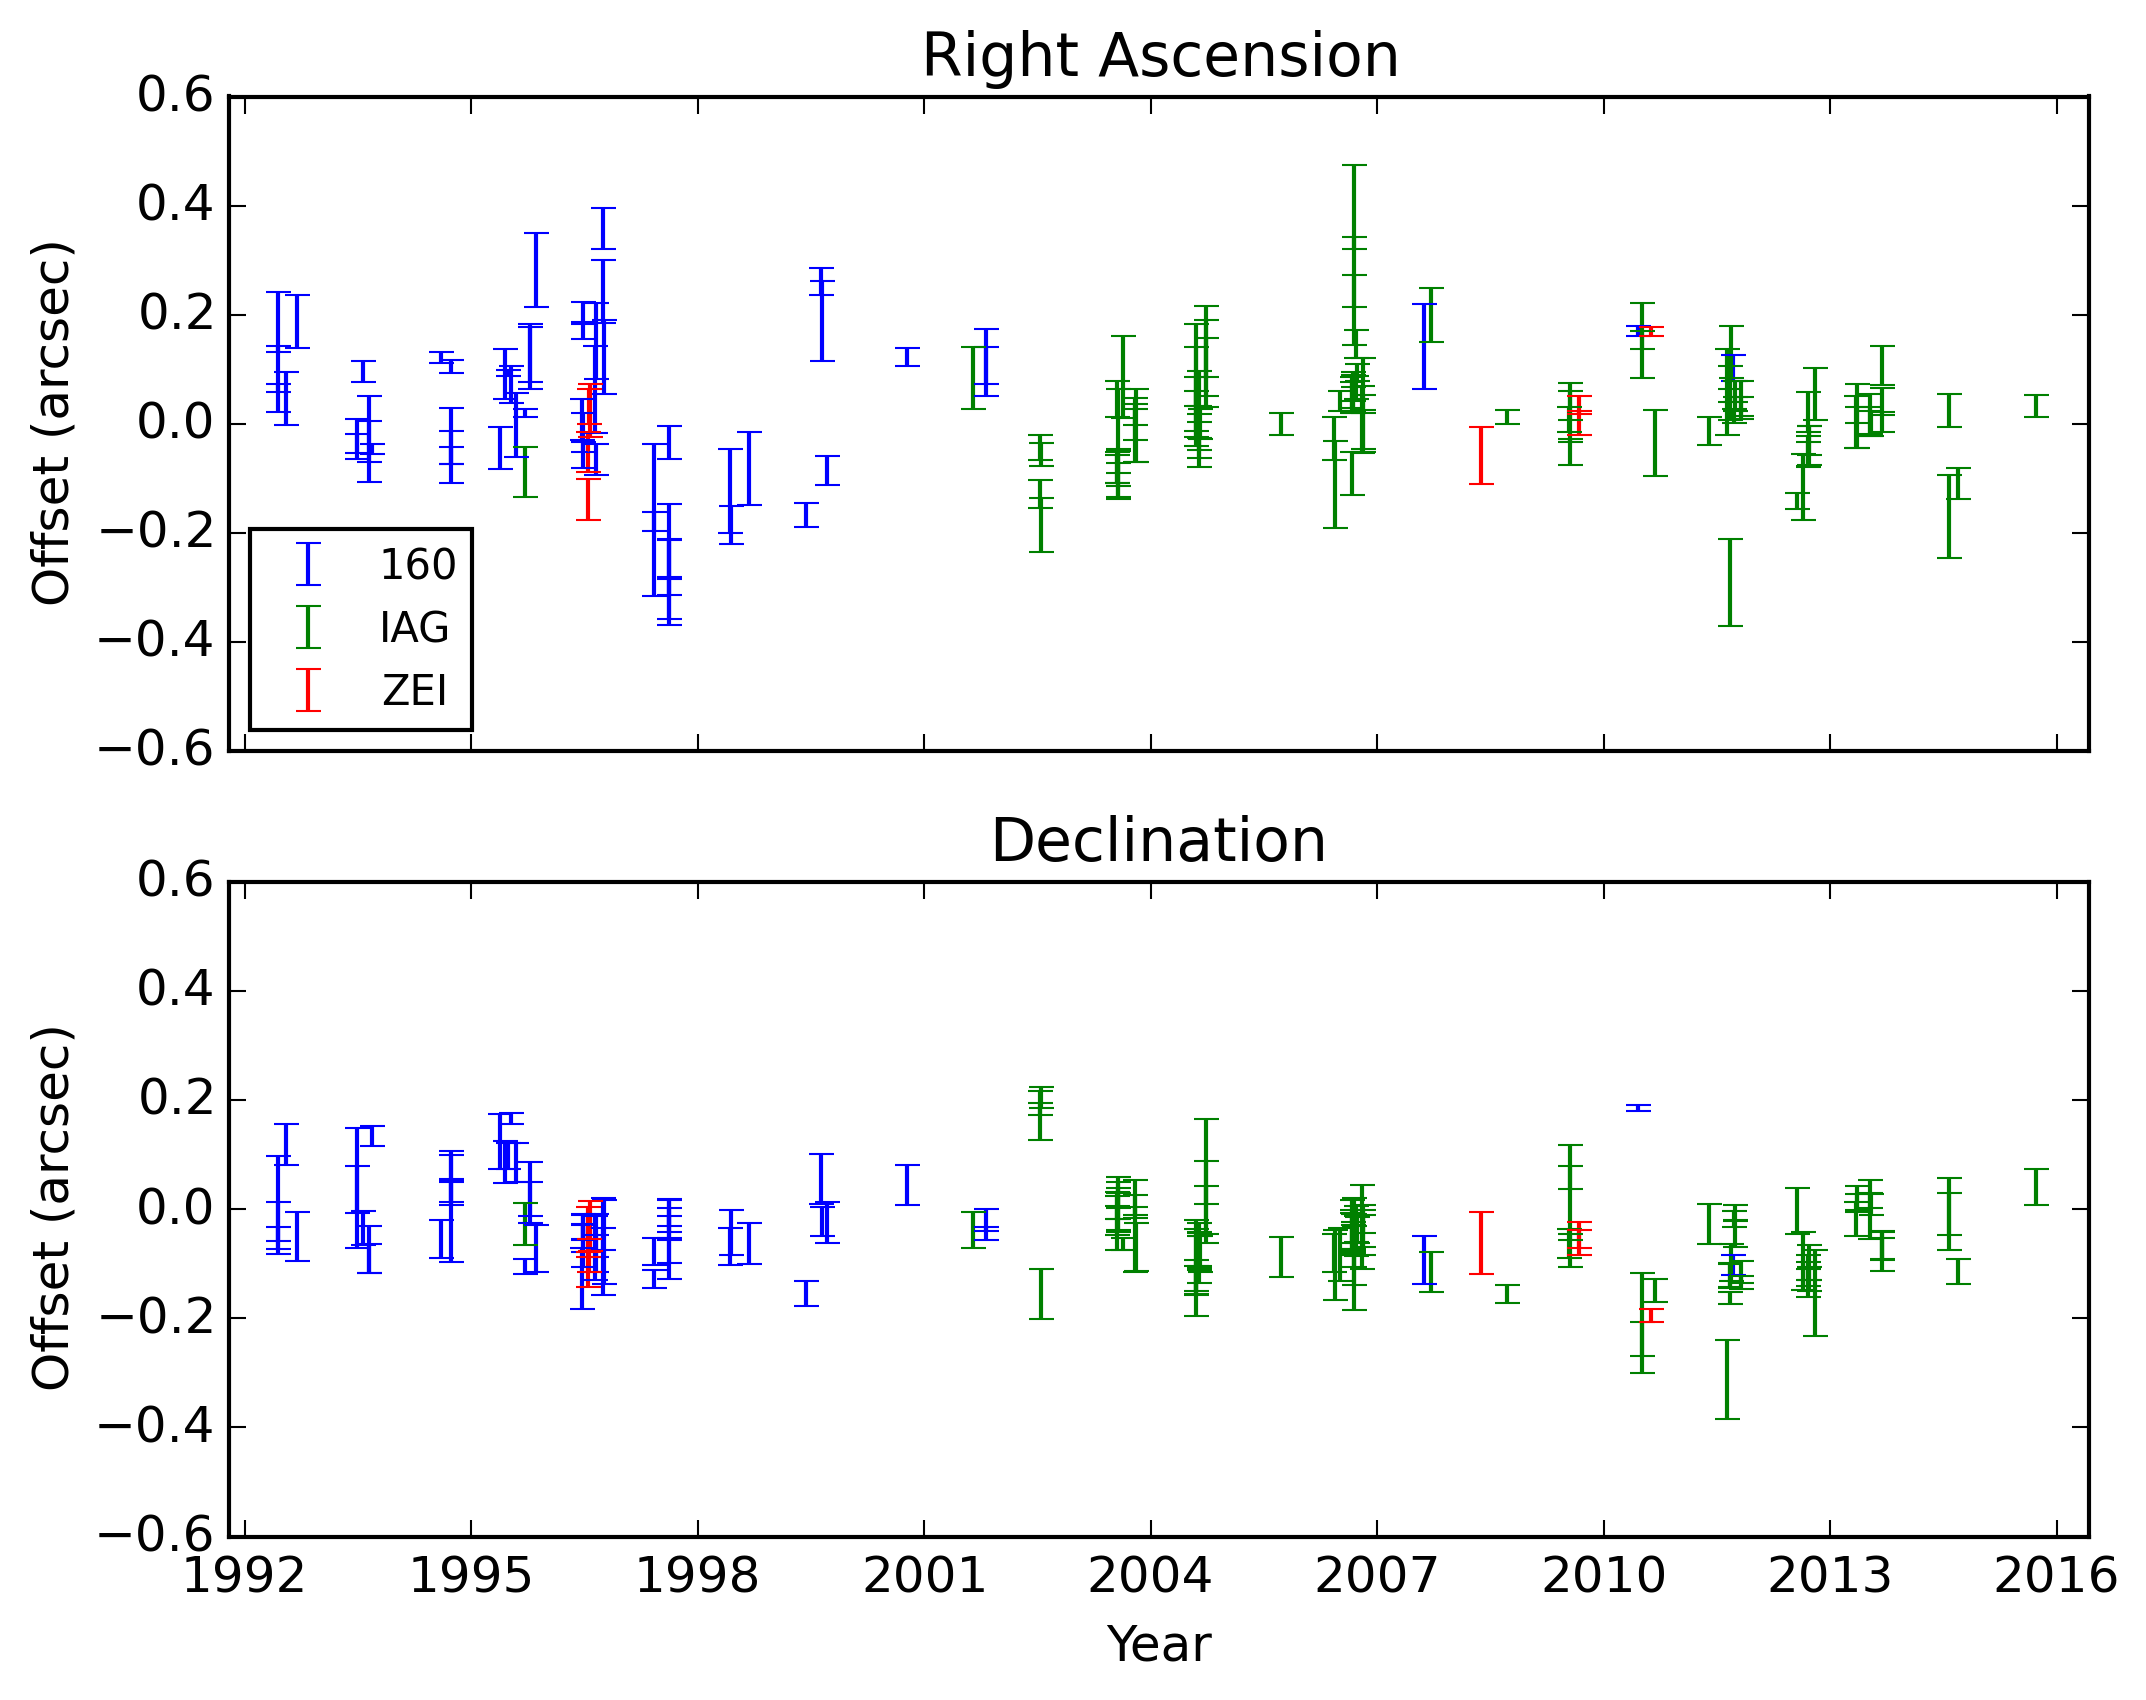
\includegraphics[width=16.0cm]{Netuno_media.png} 
\caption{Neptune - Mean offsets by day}
\label{Fig:netuno-media}
\end{figure}
\begin{figure}
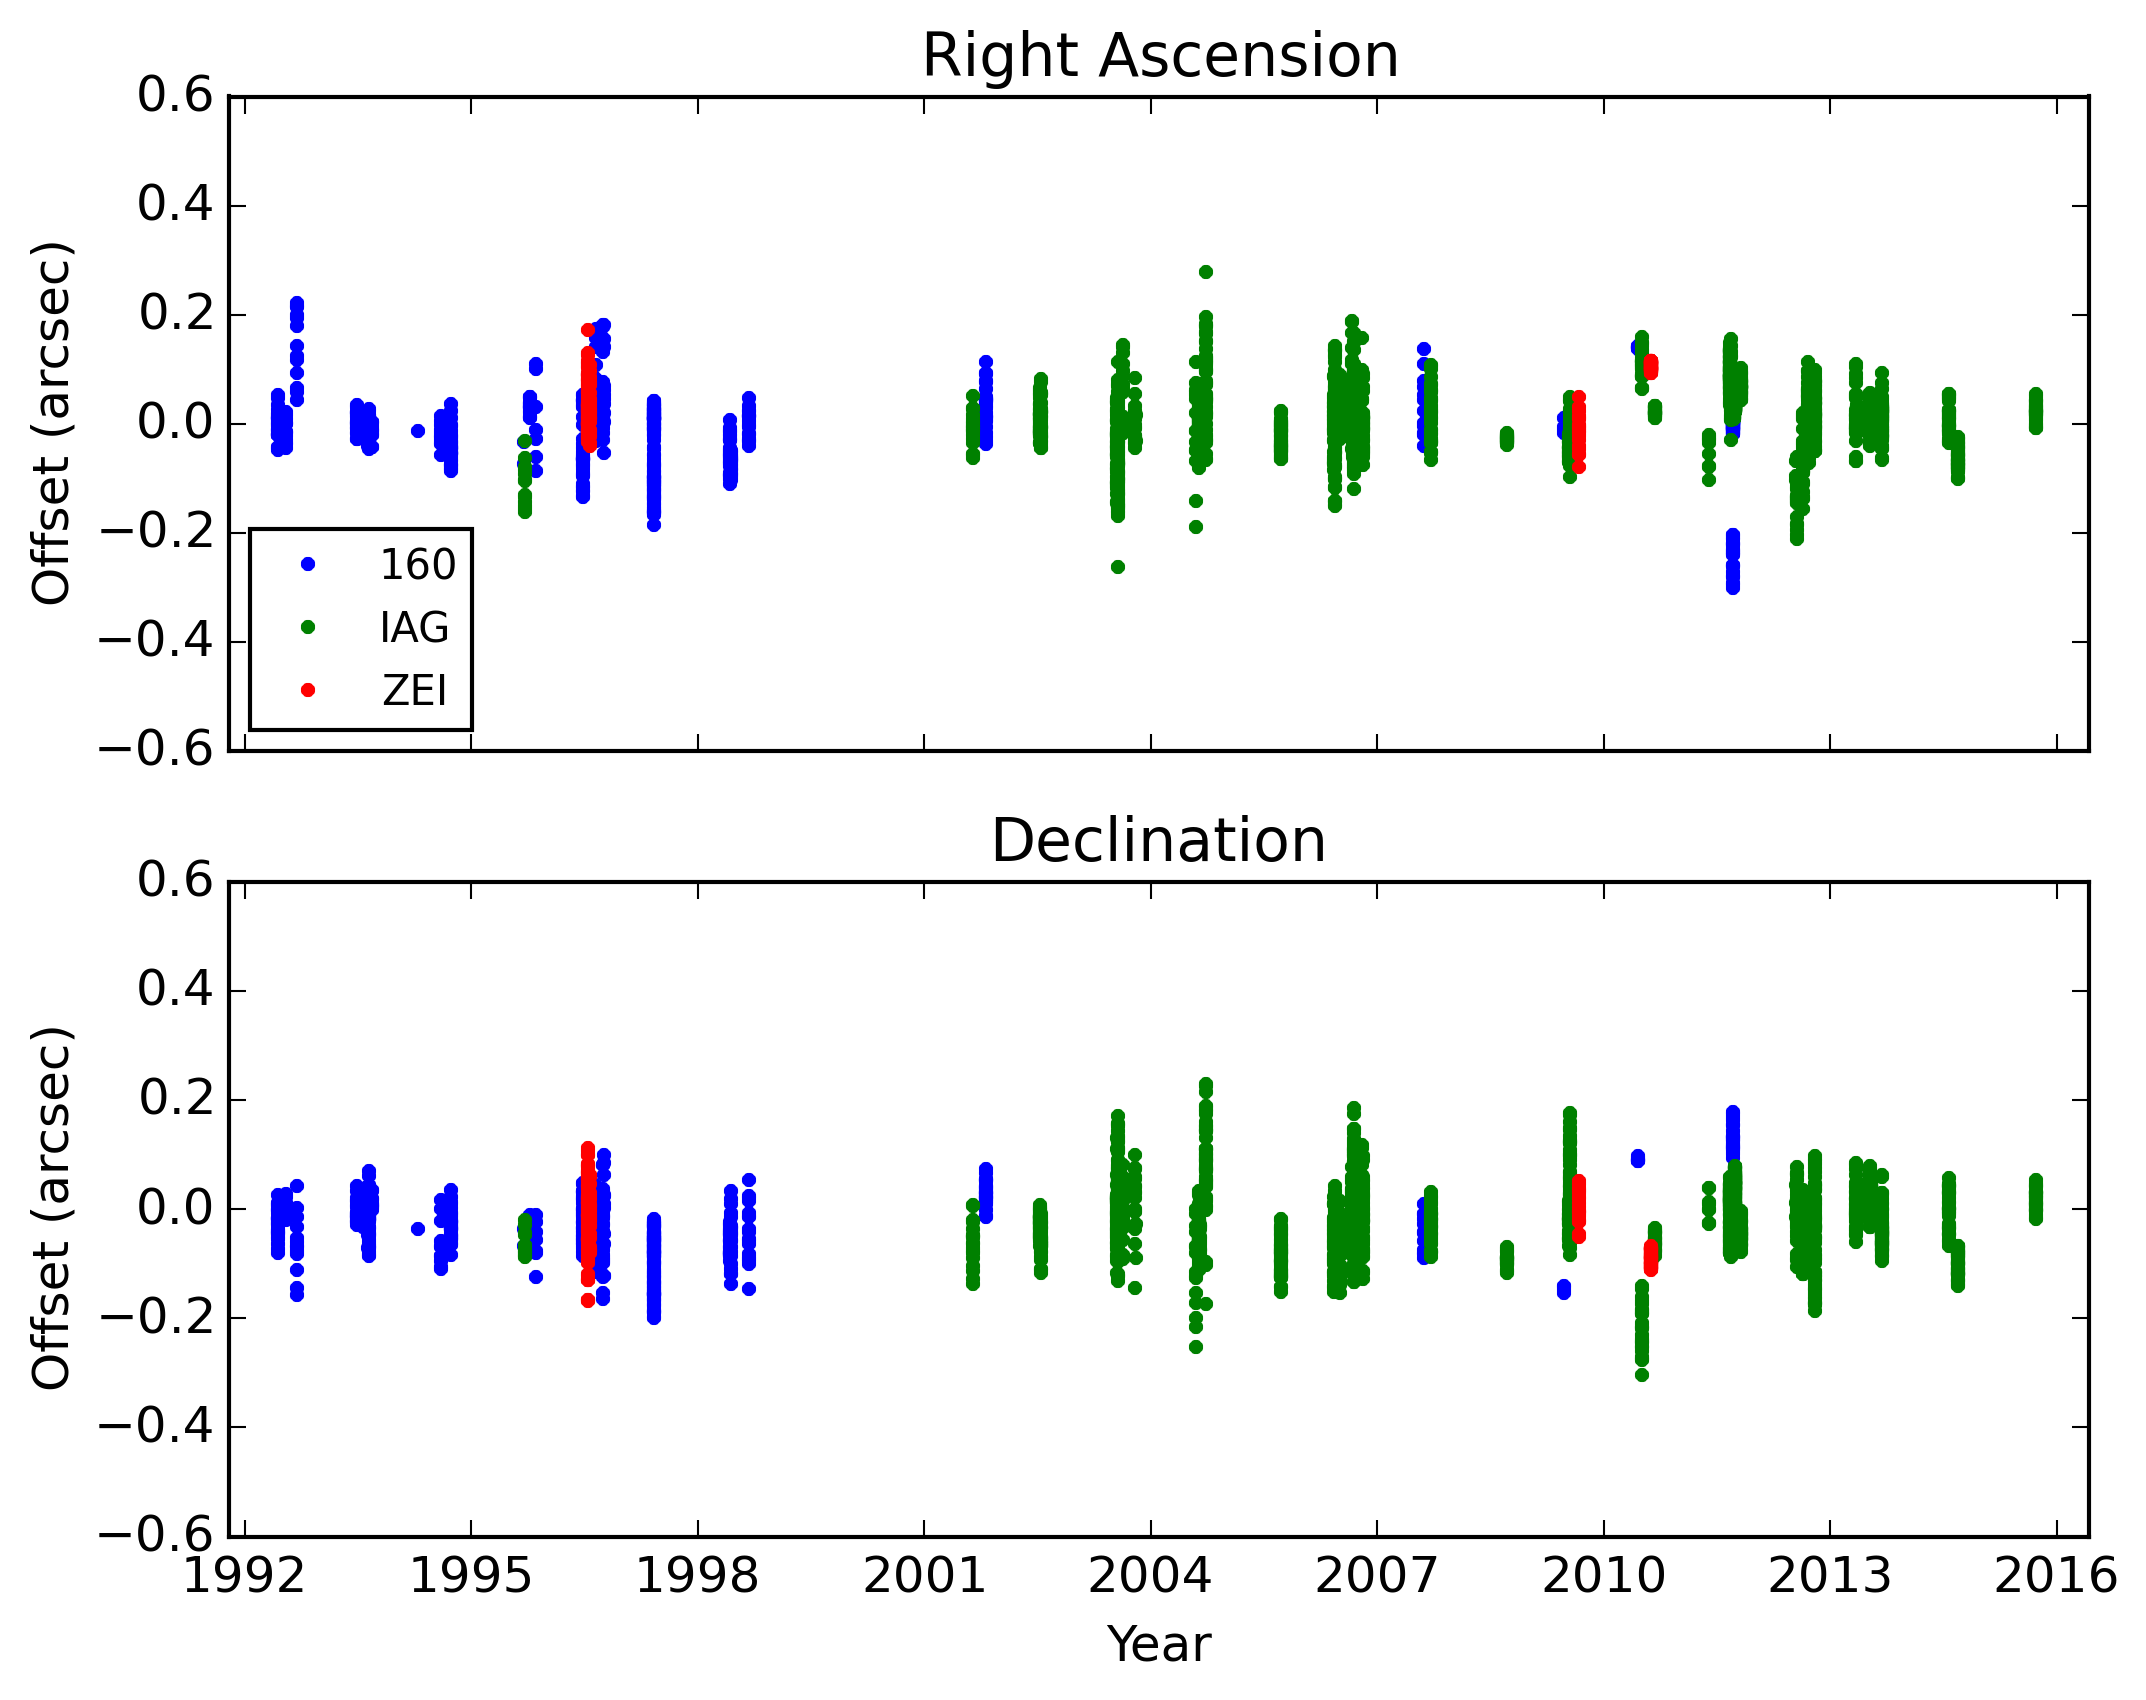
\includegraphics[width=16.0cm]{Triton_all.png} 
\caption{Triton - All Offsets}
\label{Fig:triton-all}
\end{figure}
\begin{figure}
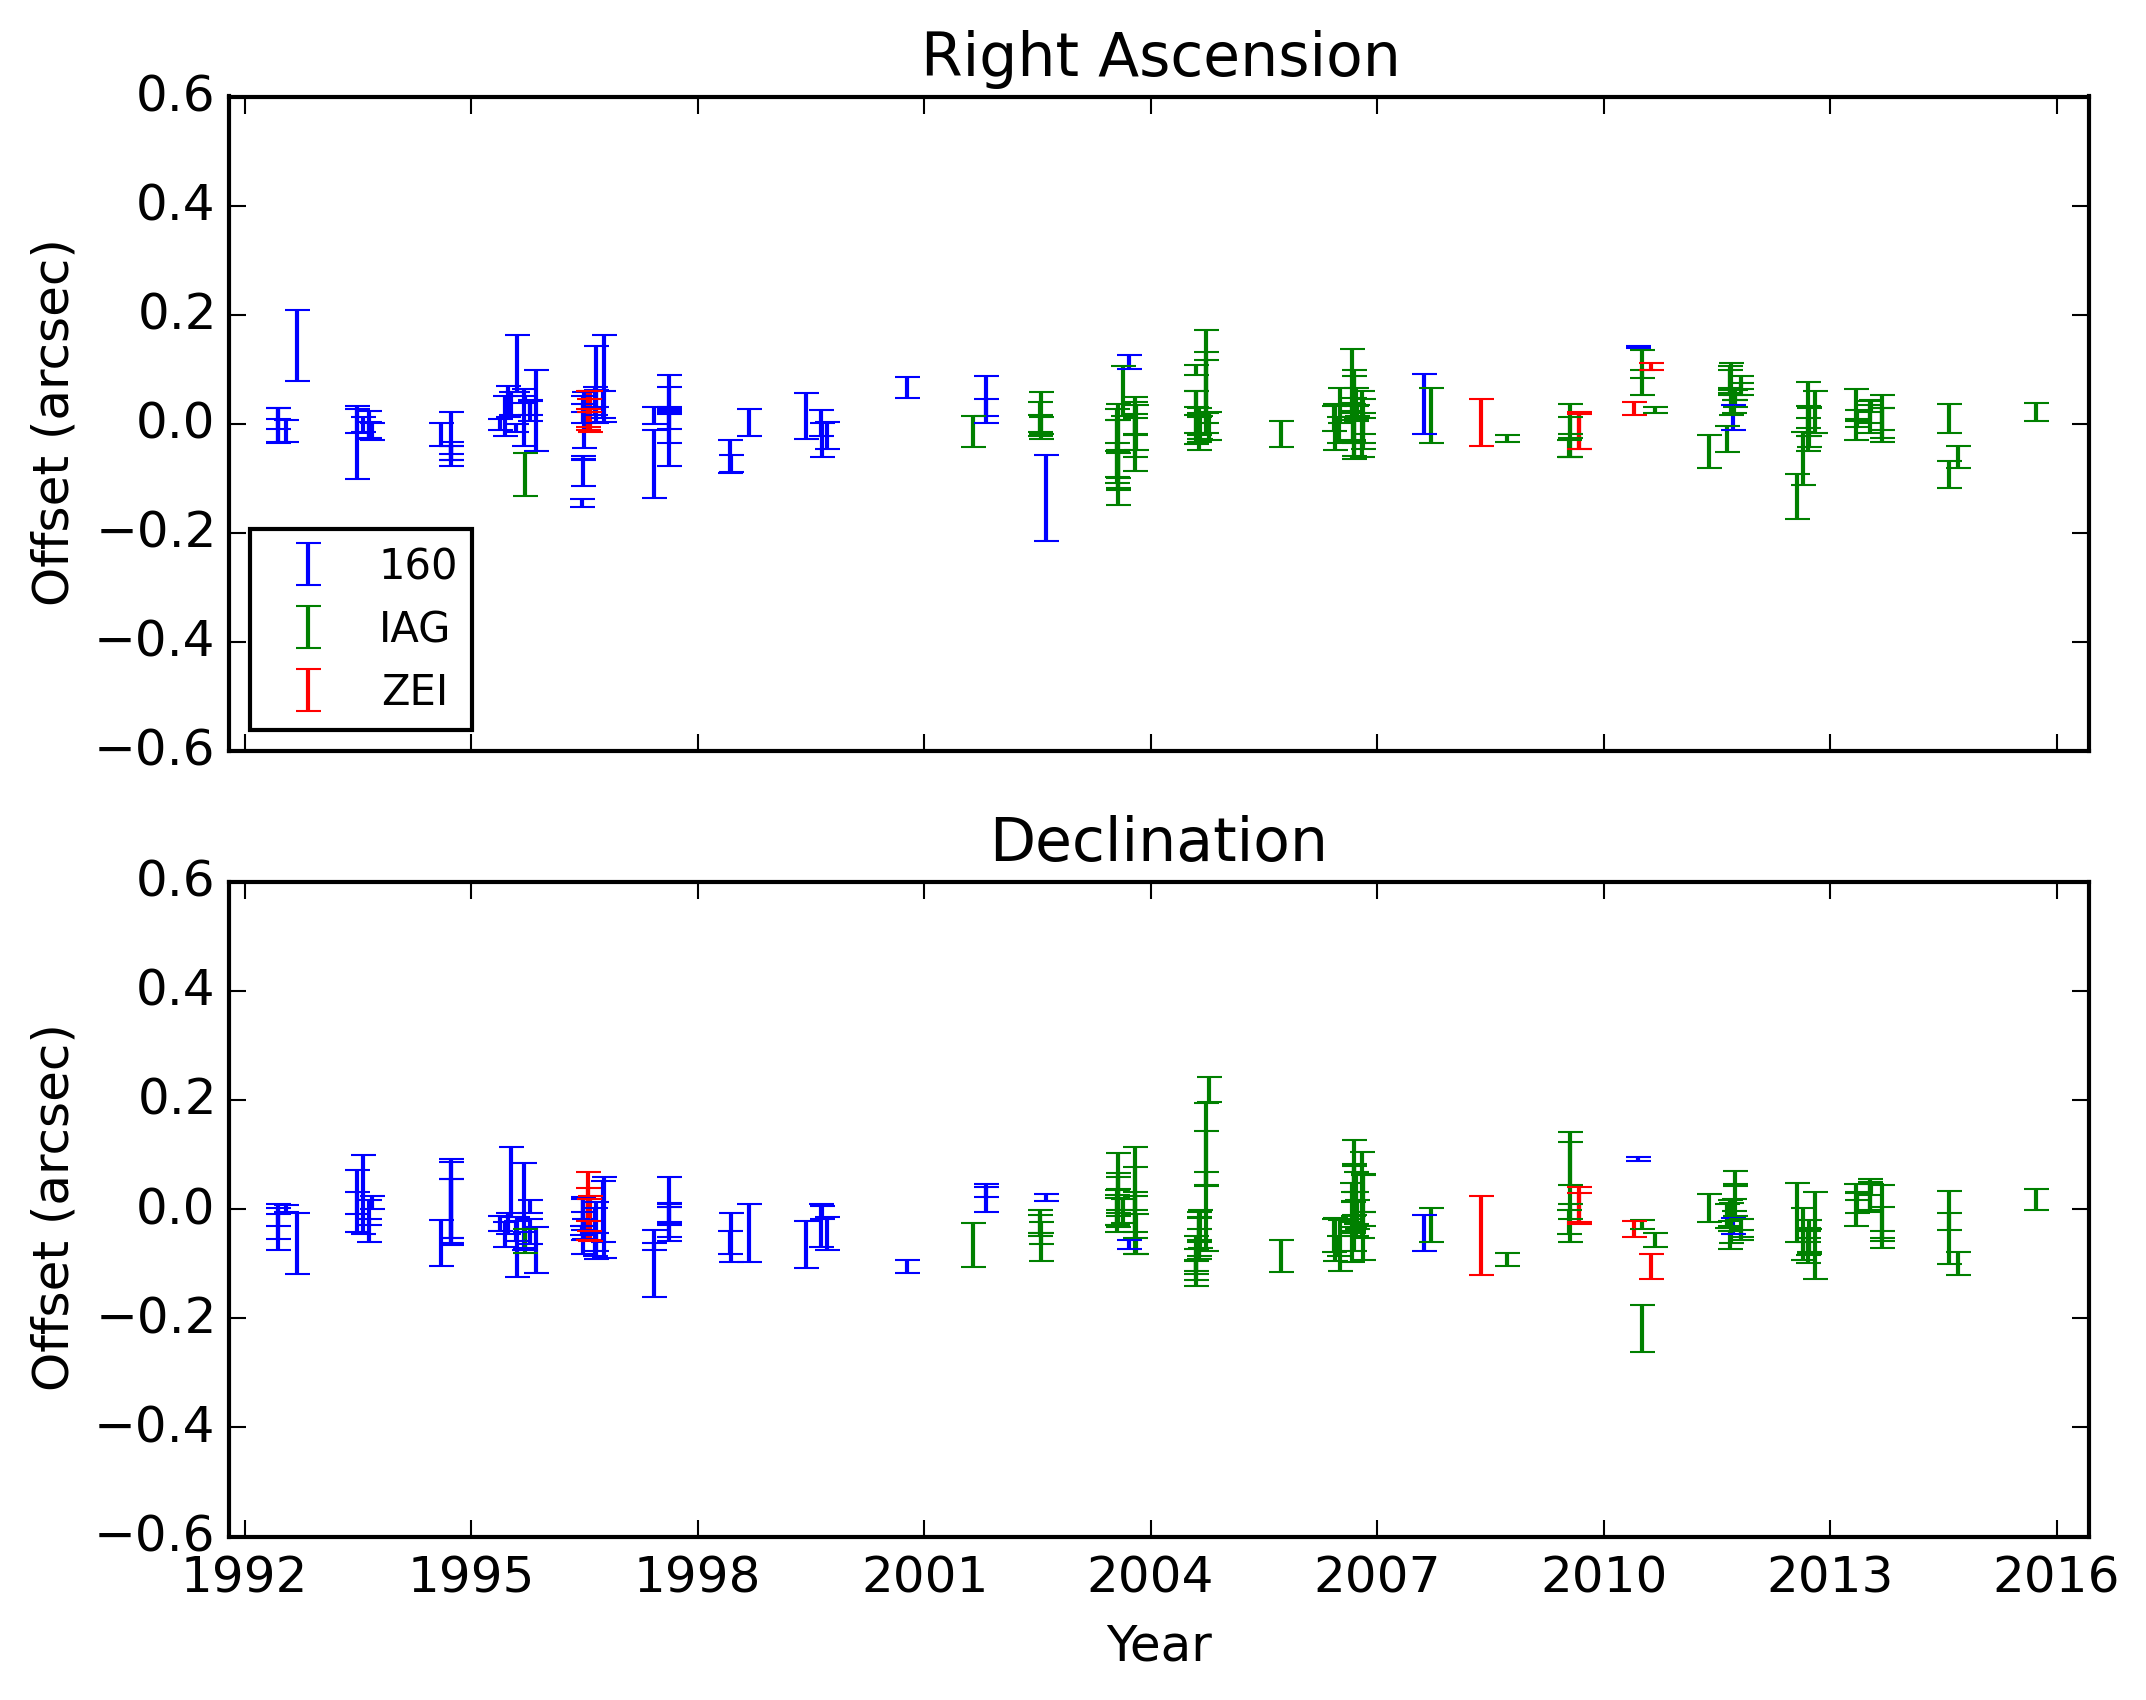
\includegraphics[width=16.0cm]{Triton_media.png} 
\caption{Triton - Mean offsets by day}
\label{Fig:trito-media}
\end{figure}
\begin{figure}
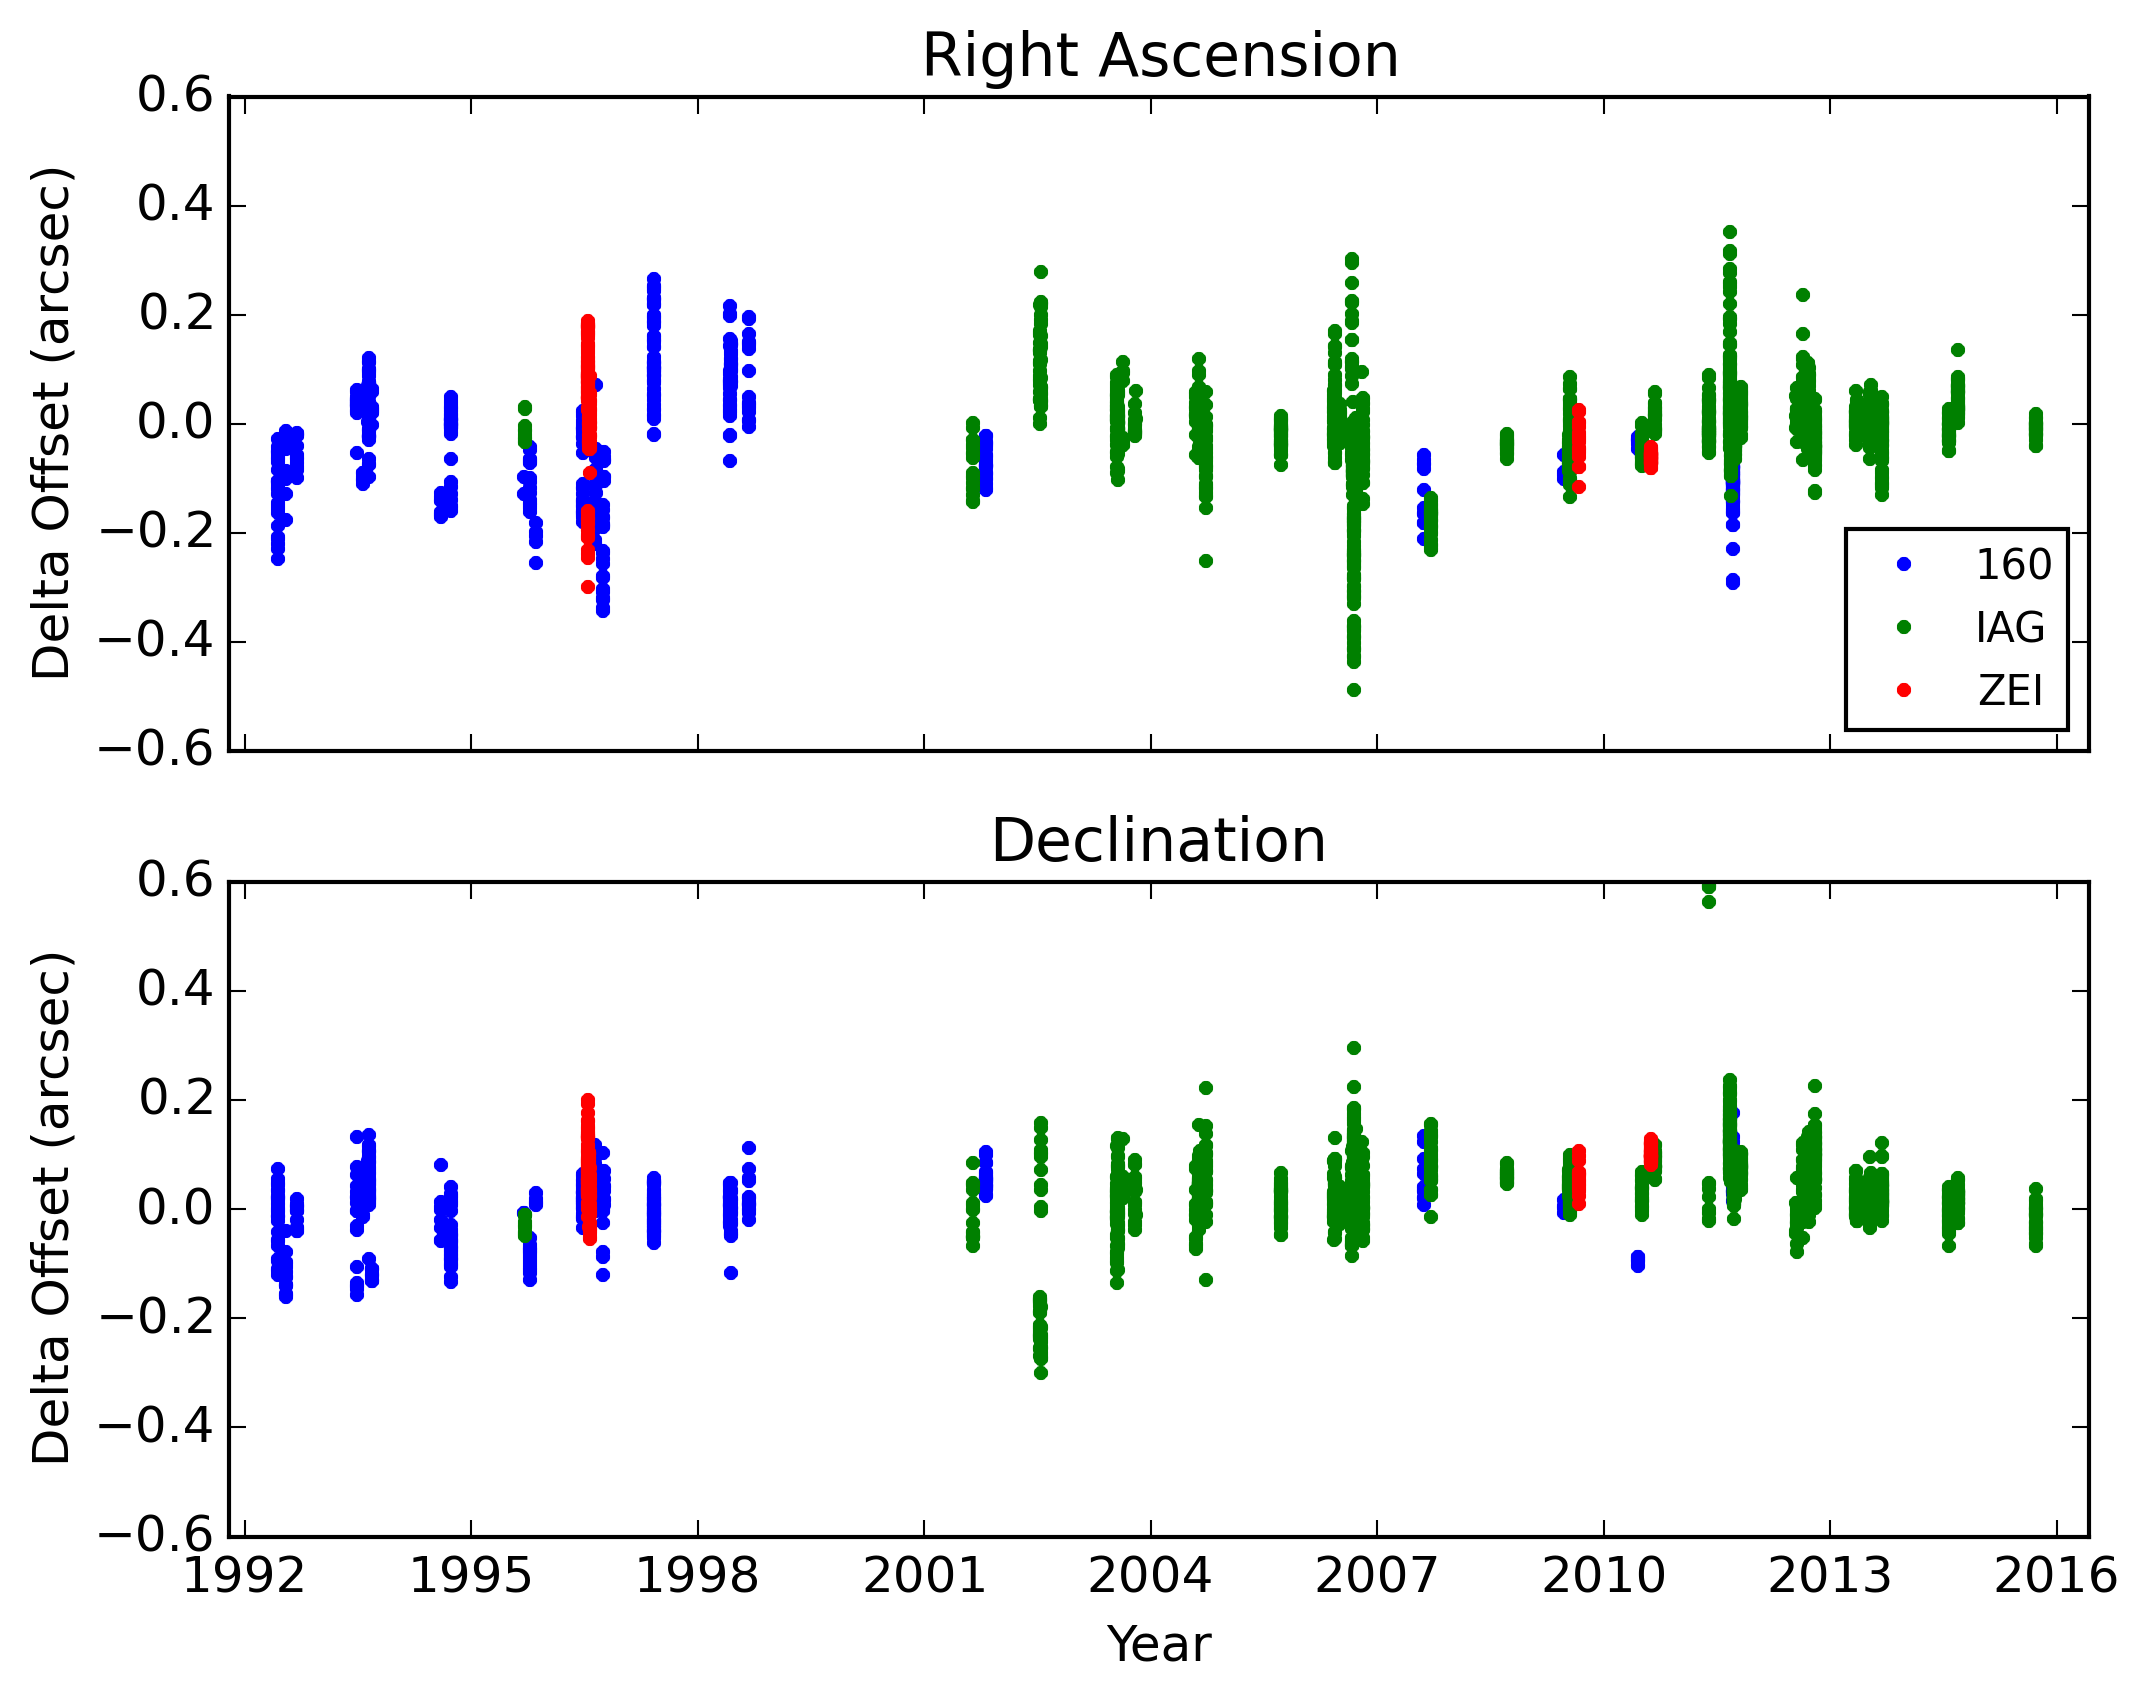
\includegraphics[width=16.0cm]{Triton-Netuno_all.png} 
\caption{Difference between the offsets of Triton and Neptune - All data}
\label{Fig:triton-netuno-all}
\end{figure}
\begin{figure}
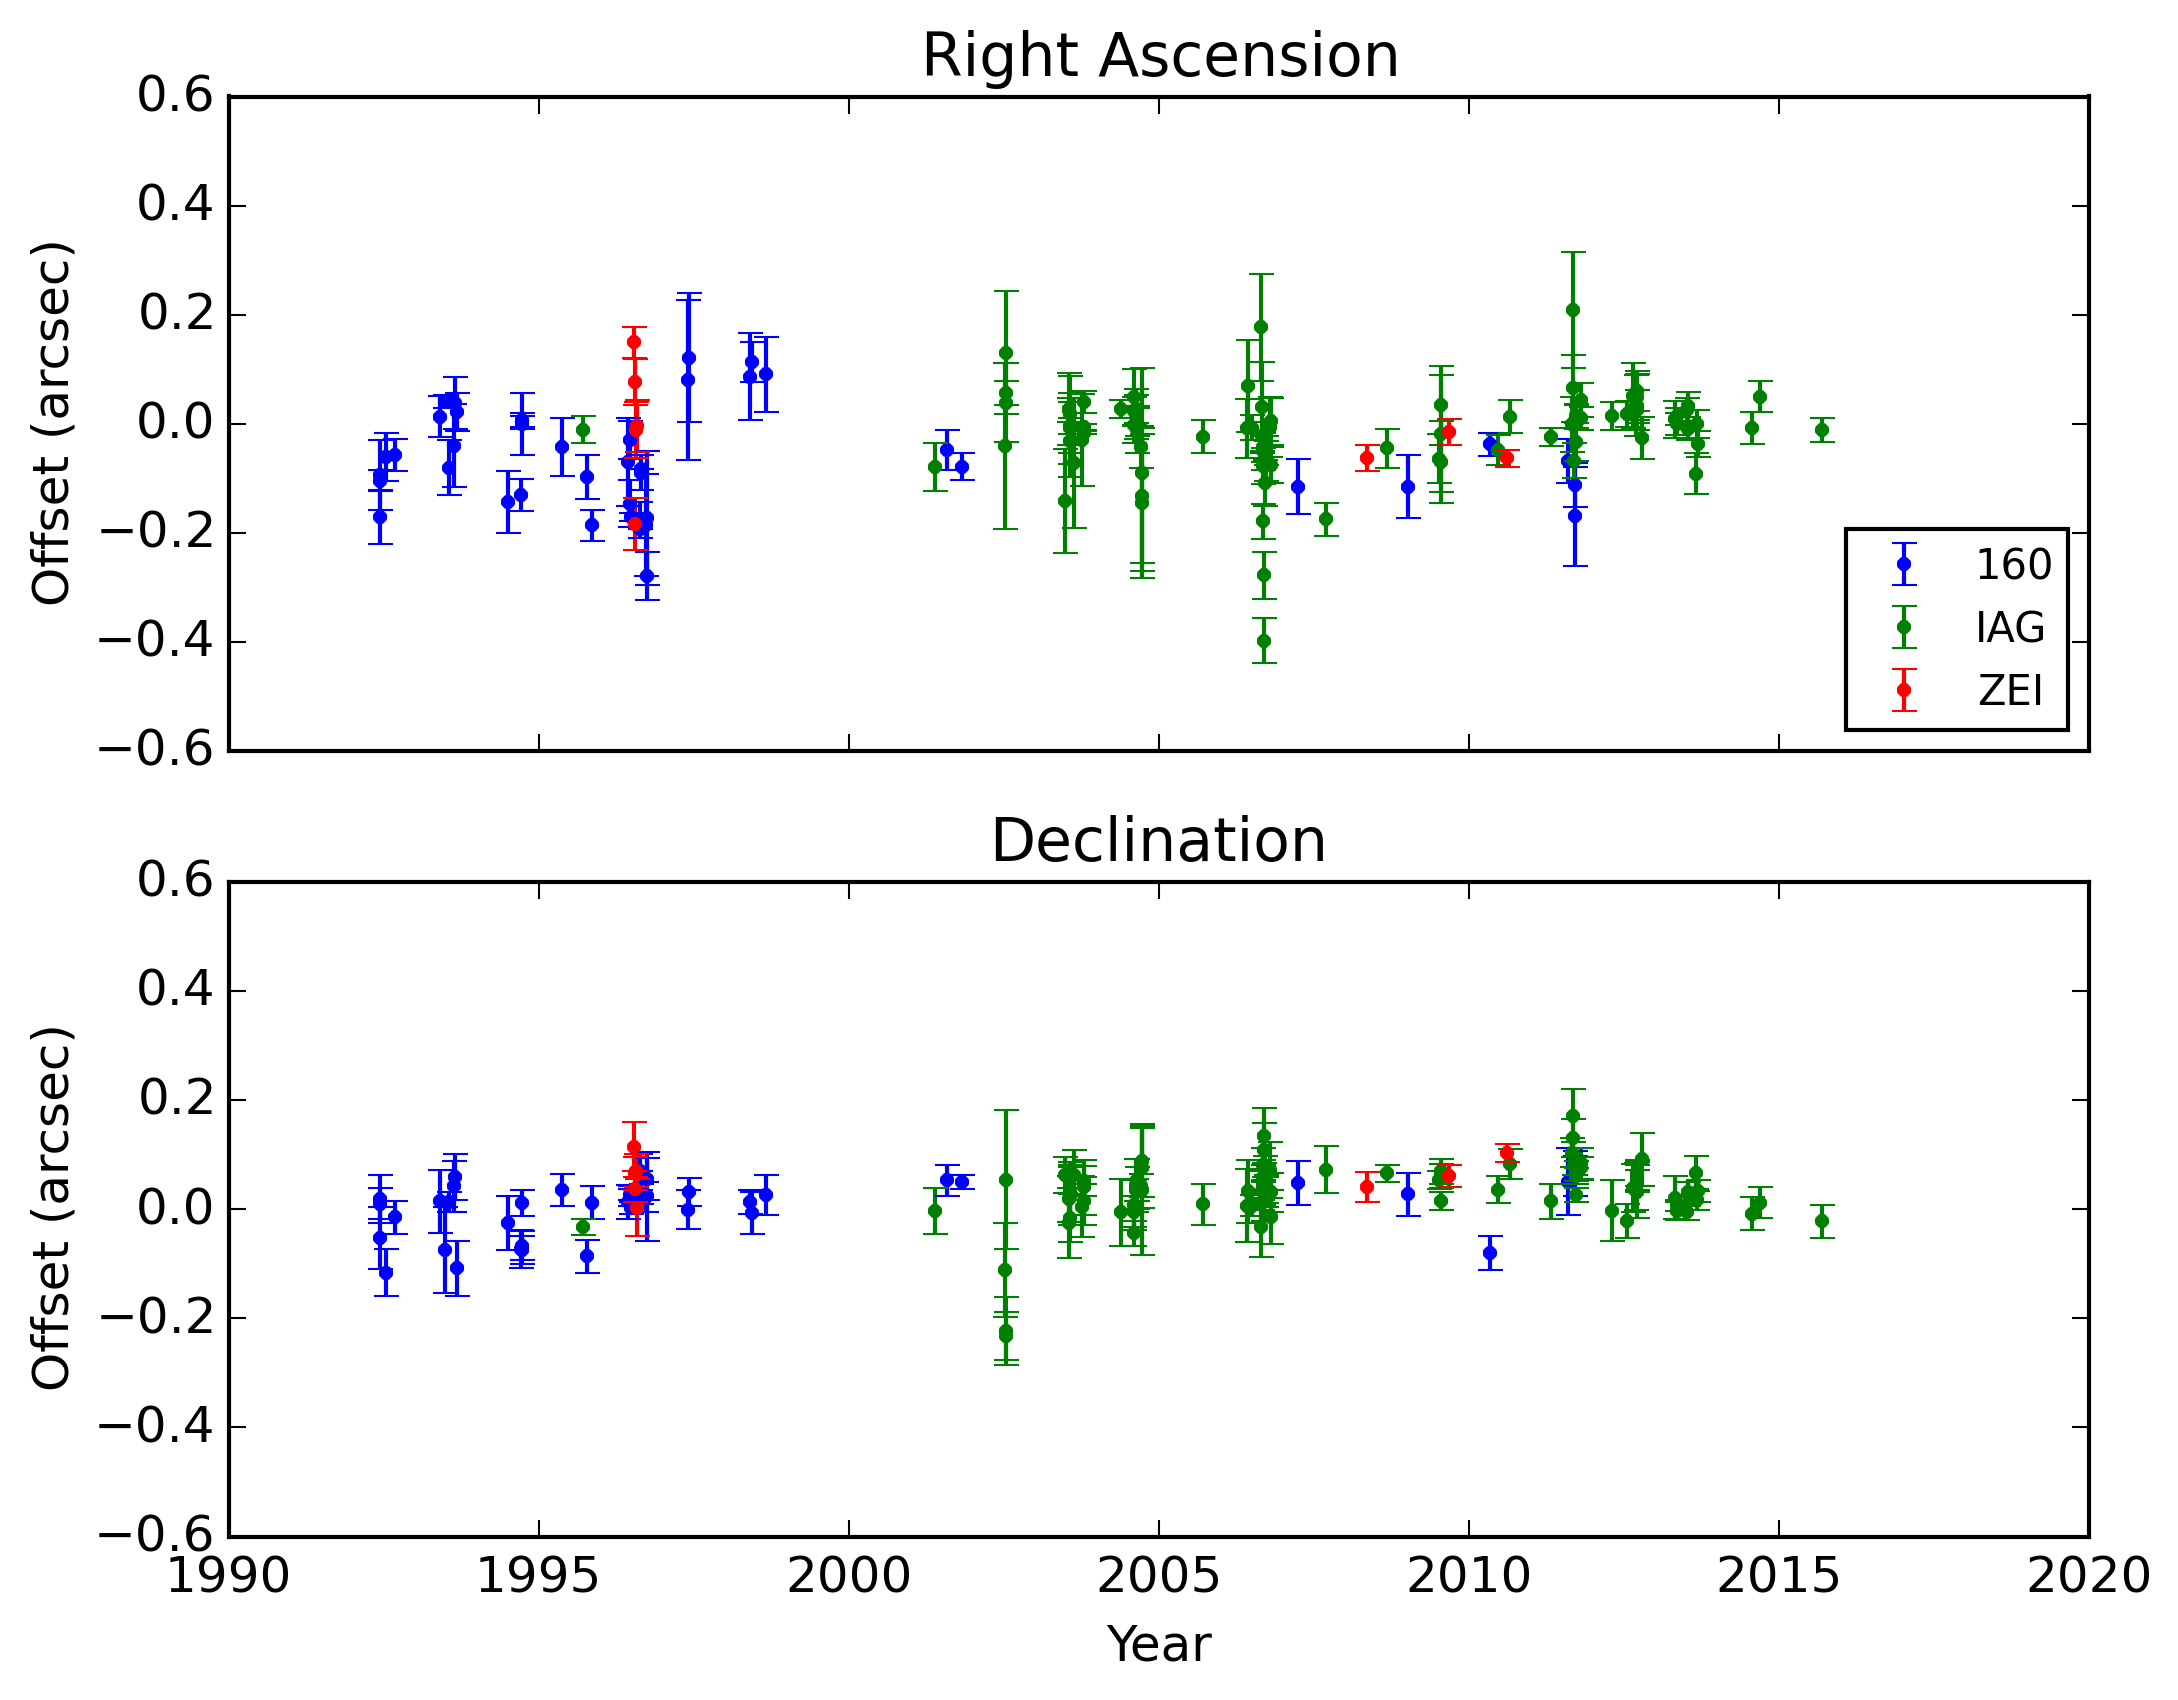
\includegraphics[width=16.0cm]{Triton-Netuno_media.png} 
\caption{Difference between the offsets of Triton and Neptune - Mean offset by day}
\label{Fig:triton-netuno-mean}
\end{figure}

%\section*{160}

\begin{figure}
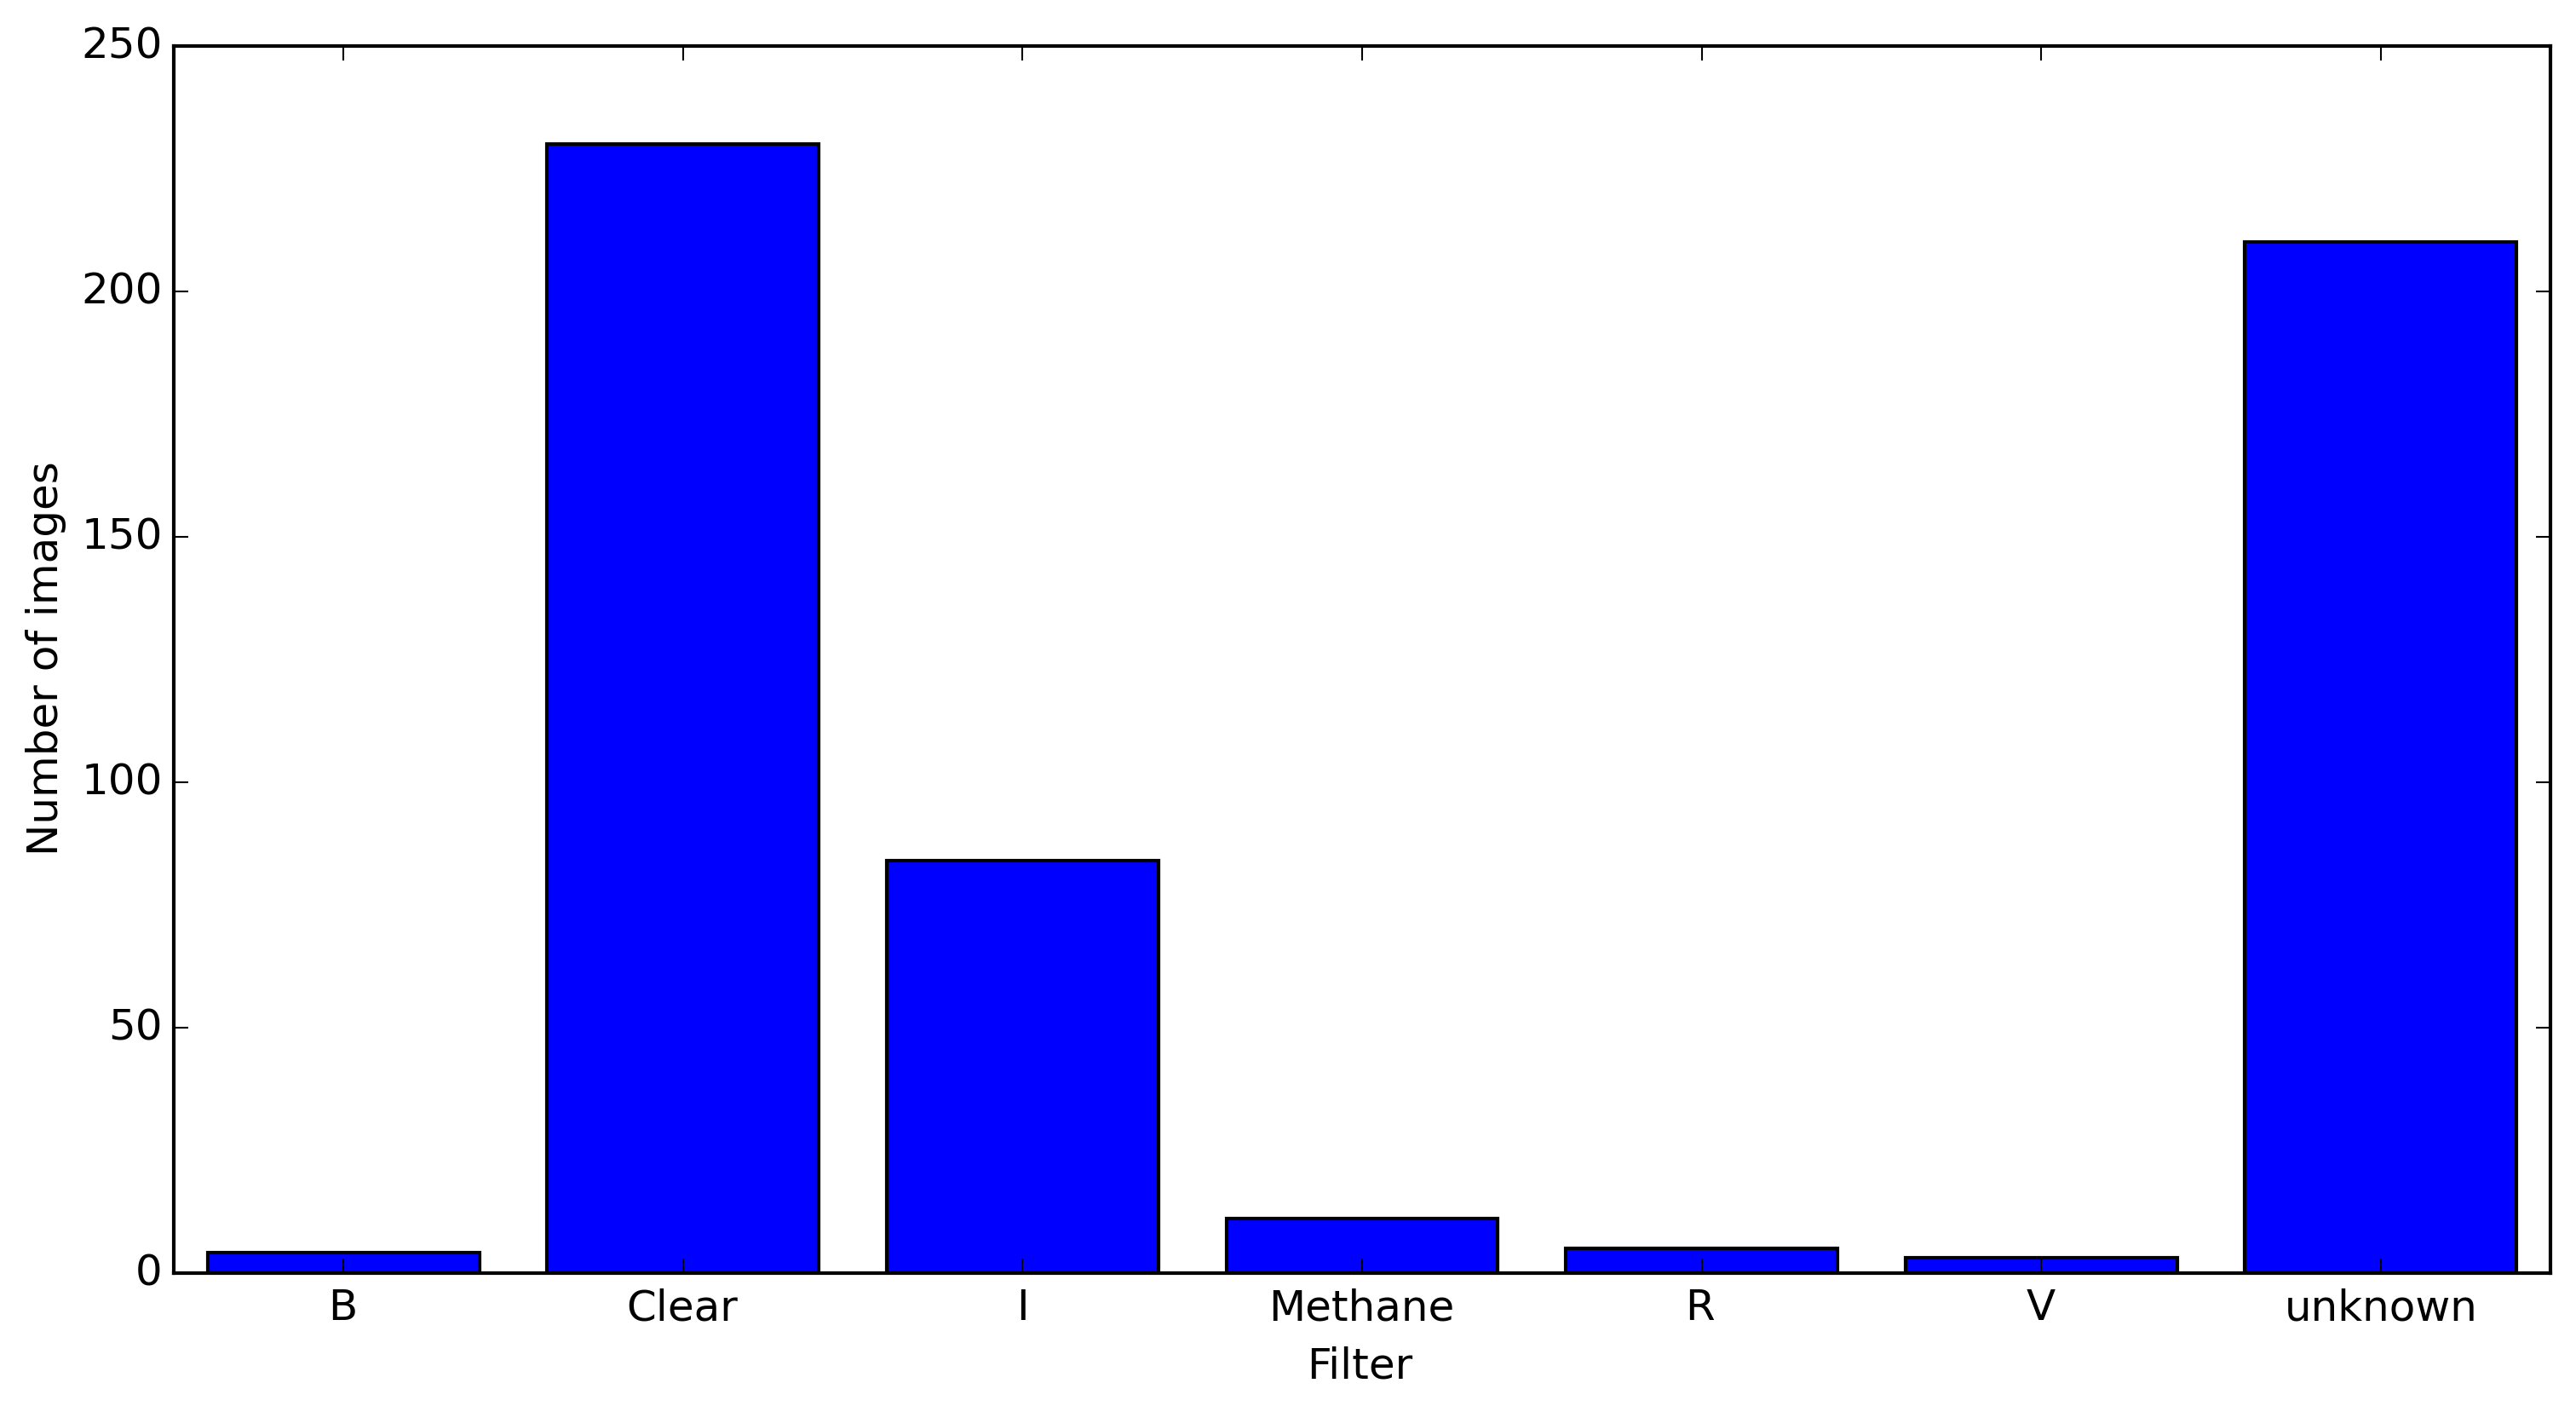
\includegraphics[width=16.0cm]{filtro_160.png} 
\caption{Distribution of positions by filter for the \PE telescope.}
\label{Fig:filtro-160}
\end{figure}

%\begin{longtable}{|c|c|c|c|c|c|c|}
%\caption{Mean offsets of Neptune night by night observed in the \PE telescope. Off-ra: mean offset em Right Ascension (mas). Off-de: mean offset in Declination (mas). E-ra: Dispersion (standard deviation) of the offsets in RA (mas). E-de: Dispersion in DEC (mas). Nfr: Number of observations per night. Date: the mean date of the observations. Ncat: average number of reference stars by frame.}\\
%\hline
%Off-ra &  Off-de &   E-ra &   E-de & Nfr & Date & Ncat \\
%\hline
%\endfirsthead
%\multicolumn{7}{c}%
%{\tablename\ \thetable\ -- \textit{Continued from previous page}} \\
%\hline
%off-ra &  off-de &   E-ra &   E-de & Nfr & Date & Ncat \\
%\hline
%\endhead
%\hline \multicolumn{7}{r}{\textit{Continued on next page}} \\
%\endfoot
%\hline
%\endlastfoot
%186.4 & 19.4 & 55.0 & 77.9 &  14 & 1992-06-09 07:51:19 & 10.0 \\
%47.7 & -52.6 & 25.5 & 19.6 &  11 & 1992-06-10 06:21:37 & 33.0 \\
%101.0 & -34.0 & 42.1 & 47.4 &   6 & 1992-06-11 06:45:25 & 16.0 \\
%46.6 & 118.8 & 48.0 & 37.8 &  18 & 1992-07-19 03:23:22 & 23.0 \\
%187.9 & -49.6 & 48.3 & 45.2 &  15 & 1992-09-11 01:11:36 & 25.0 \\
%-22.5 & 4.0 & 31.1 & 75.6 &  15 & 1993-06-24 04:32:16 & 16.0 \\
%-41.9 & 70.5 & 22.6 & 78.2 &  12 & 1993-06-25 04:43:38 & 9.0 \\
%95.0 & -33.9 & 19.2 & 30.8 &   7 & 1993-07-27 04:00:31 & 23.0 \\
%-10.0 & -90.0 & 60.6 & 26.6 &  24 & 1993-08-21 00:31:24 & 29.0 \\
%-50.6 & -73.9 & 55.6 & 43.9 &  35 & 1993-08-22 23:36:48 & 9.0 \\
%-46.7 & 133.9 & 9.3 & 18.5 &  11 & 1993-09-06 22:33:58 & 9.0 \\
%121.9 & -54.4 & 10.5 & 35.2 &   8 & 1994-08-05 04:13:11 & 15.0 \\
%104.9 & 78.0 & 11.7 & 28.6 &   8 & 1994-09-22 00:43:05 & 11.0 \\
%-39.5 & 54.0 & 69.3 & 46.3 &  13 & 1994-09-22 22:46:08 & 24.0 \\
%-57.4 & 32.9 & 15.7 & 19.8 &  10 & 1994-09-23 23:11:52 & 26.0 \\
%-43.5 & -20.4 & 30.0 & 76.1 &  13 & 1994-09-24 22:43:01 & 27.0 \\
%-43.8 & 124.2 & 38.5 & 50.4 &  10 & 1995-05-19 07:11:17 & 11.0 \\
%91.6 & 86.9 & 45.3 & 38.1 &  14 & 1995-06-13 06:09:42 & 13.0 \\
%93.4 & 97.8 & 5.4 & 23.3 &  10 & 1995-06-27 05:34:17 & 8.0 \\
%71.3 & 166.3 & 33.8 & 10.0 &   9 & 1995-07-11 03:37:19 & 17.0 \\
%-2.1 & 85.3 & 58.1 & 35.7 &  10 & 1995-08-07 01:38:00 & 21.0 \\
%19.2 & -104.3 & 7.6 & 13.6 &  15 & 1995-09-17 00:36:24 & 14.0 \\
%127.2 & 30.9 & 50.1 & 55.4 &  25 & 1995-10-11 23:16:34 & 23.0 \\
%123.0 & 19.0 & 60.0 & 31.0 &   4 & 1995-10-12 22:54:50 & 13.0 \\
%281.9 & -72.0 & 68.5 & 42.7 &   8 & 1995-11-10 22:46:56 & 6.0 \\
%7.8 & -127.4 & 38.3 & 56.2 &  16 & 1996-06-21 06:20:04 & 13.0 \\
%-30.0 & -40.2 & 50.6 & 13.7 &  13 & 1996-06-22 05:17:12 & 15.0 \\
%-43.1 & -42.2 & 8.8 & 13.8 &  17 & 1996-06-23 05:11:07 & 11.0 \\
%203.3 & -44.8 & 20.3 & 34.1 &  11 & 1996-06-24 06:57:46 & 12.0 \\
%171.0 & -57.6 & 16.2 & 48.8 &   5 & 1996-06-25 06:46:08 & 15.0 \\
%63.1 & -71.7 & 79.6 & 58.9 &  19 & 1996-08-22 03:18:27 & 13.0 \\
%152.6 & -48.1 & 69.6 & 40.1 &   9 & 1996-08-24 03:47:49 & 8.0 \\
%-65.6 & -81.8 & 28.6 & 33.9 &  12 & 1996-08-25 01:03:19 & 10.0 \\
%243.1 & -26.8 & 58.0 & 47.2 &  11 & 1996-09-28 01:32:28 & 7.0 \\
%358.3 & -95.2 & 37.8 & 61.3 &  12 & 1996-09-29 02:18:58 & 12.0 \\
%123.0 & -60.1 & 67.8 & 76.4 &   8 & 1996-10-02 00:27:18 & 5.0 \\
%-238.5 & -127.4 & 76.6 & 16.4 &  40 & 1997-06-01 05:10:31 & 10.0 \\
%-116.2 & -77.6 & 79.9 & 25.4 &  41 & 1997-06-02 05:47:21 & 9.0 \\
%-290.4 & -17.6 & 77.6 & 35.4 &  34 & 1997-08-12 00:34:48 & 10.0 \\
%-34.3 & -6.4 & 31.1 & 24.8 &  15 & 1997-08-13 03:08:20 & 9.0 \\
%-216.2 & -19.8 & 68.7 & 22.4 &  19 & 1997-08-13 23:57:27 & 5.0 \\
%-284.3 & -70.5 & 73.0 & 57.3 &  20 & 1997-08-14 23:49:36 & 6.0 \\
%-297.4 & -77.9 & 16.0 & 20.8 &  17 & 1997-08-15 23:17:19 & 14.0 \\
%-123.9 & -68.9 & 77.2 & 33.8 &  30 & 1998-06-06 05:10:18 & 11.0 \\
%-185.2 & -41.8 & 34.4 & 41.2 &  24 & 1998-06-08 04:20:38 & 19.0 \\
%-82.7 & -63.3 & 66.8 & 37.5 &  18 & 1998-09-03 23:01:05 & 10.0 \\
%-167.1 & -154.2 & 22.6 & 23.2 &  10 & 1999-06-06 04:38:42 & 12.0 \\
%260.6 & 55.5 & 24.8 & 46.2 &   8 & 1999-08-21 04:13:56 & 17.0 \\
%188.1 & -22.1 & 73.6 & 26.9 &  17 & 1999-08-22 03:35:44 & 14.0 \\
%-85.6 & -24.0 & 26.3 & 37.6 &  18 & 1999-09-17 22:47:52 & 10.0 \\
%122.7 & 44.8 & 16.7 & 37.0 &  20 & 2000-10-09 23:56:21 & 9.0 \\
%106.9 & -44.5 & 34.0 & 12.1 &  13 & 2001-10-24 22:46:18 & 5.0 \\
%112.2 & -20.3 & 61.7 & 20.4 &  18 & 2001-10-27 22:38:36 & 9.0 \\
%141.9 & -92.7 & 77.6 & 44.4 &  14 & 2007-08-17 06:39:00 & 6.0 \\
%170.3 & 185.6 & 9.0 & 6.3 &   8 & 2010-06-16 08:52:32 & 5.0 \\
%102.7 & -101.8 & 23.5 & 18.5 &  60 & 2011-09-20 02:04:26 & 5.0 \\
%\hline
%\end{longtable}
%
%\begin{longtable}{|c|c|c|c|c|c|c|}
%\caption{Same as in Table 2 for Triton in the \PE telescope.}\\
%\hline
%Off-ra &  Off-de &   E-ra &   E-de & Nfr & Date & Ncat \\
%\hline
%\endfirsthead
%\multicolumn{7}{c}%
%{\tablename\ \thetable\ -- \textit{Continued from previous page}} \\
%\hline
%off-ra &  off-de &   E-ra &   E-de & Nfr & Date & Ncat \\
%\hline
%\endhead
%\hline \multicolumn{7}{r}{\textit{Continued on next page}} \\
%\endfoot
%\hline
%\endlastfoot
%9.5 & -14.2 & 19.2 & 16.5 &  13 & 1992-06-09 07:49:08 &  11 \\
%-12.7 & -31.5 & 21.3 & 23.4 &  11 & 1992-06-10 06:20:08 &  30 \\
%-3.8 & -32.3 & 31.9 & 41.7 &   6 & 1992-06-11 06:45:25 &  16 \\
%-13.2 & 2.0 & 21.0 & 6.2 &  12 & 1992-07-19 03:28:00 &  23 \\
%143.8 & -63.2 & 64.5 & 55.7 &  13 & 1992-09-11 01:11:58 &  24 \\
%8.0 & 15.3 & 24.0 & 57.3 &  15 & 1993-06-24 03:57:40 &  12 \\
%-37.6 & 10.8 & 63.8 & 20.4 &  16 & 1993-06-25 05:04:44 &  12 \\
%-1.1 & 27.2 & 14.0 & 72.7 &  10 & 1993-07-27 04:03:11 &  23 \\
%-11.7 & -39.4 & 15.8 & 21.5 &  20 & 1993-08-21 00:43:19 &  28 \\
%-1.8 & -5.8 & 24.6 & 22.3 &  33 & 1993-08-22 23:49:13 &  13 \\
%-14.5 & 13.0 & 15.9 & 11.8 &  12 & 1993-09-06 22:34:10 &   9 \\
%-19.6 & -61.8 & 20.7 & 42.6 &  11 & 1994-08-05 04:13:04 &  15 \\
%-22.7 & 19.7 & 43.4 & 71.6 &  12 & 1994-09-22 00:49:21 &  11 \\
%-58.8 & 9.7 & 18.4 & 76.1 &  12 & 1994-09-22 22:45:45 &  16 \\
%-53.3 & 1.7 & 13.1 & 54.6 &  15 & 1994-09-23 23:21:39 &  18 \\
%-44.4 & -3.5 & 10.9 & 58.2 &  11 & 1994-09-24 22:49:53 &  26 \\
%-1.0 & -25.9 & 9.8 & 13.4 &  10 & 1995-05-19 07:11:17 &  11 \\
%14.7 & -46.8 & 36.3 & 22.8 &  18 & 1995-06-13 06:15:21 &  14 \\
%41.6 & -26.0 & 28.3 & 18.6 &  14 & 1995-06-27 05:46:20 &   8 \\
%37.1 & 50.4 & 20.8 & 64.5 &  19 & 1995-07-11 03:53:15 &  17 \\
%-7.4 & -40.4 & 7.7 & 18.1 &   9 & 1995-08-07 02:05:10 &  21 \\
%110.6 & -69.0 & 52.1 & 54.9 &  10 & 1995-08-09 04:40:34 &   4 \\
%11.2 & 5.0 & 51.7 & 79.0 &  10 & 1995-09-14 01:41:37 &   9 \\
%43.9 & -57.0 & 6.4 & 14.8 &  18 & 1995-09-17 00:34:02 &  13 \\
%24.1 & -40.6 & 18.1 & 22.6 &  20 & 1995-10-11 23:13:27 &  23 \\
%30.2 & 4.2 & 13.8 & 11.9 &   6 & 1995-10-12 22:57:46 &  18 \\
%24.0 & -74.7 & 74.5 & 42.6 &  10 & 1995-11-10 22:48:25 &   7 \\
%-146.1 & -38.9 & 7.3 & 8.1 &  14 & 1996-06-21 06:15:10 &  15 \\
%-89.5 & -5.5 & 23.9 & 25.8 &  30 & 1996-06-22 05:31:09 &  14 \\
%-62.4 & -21.7 & 3.0 & 16.5 &  13 & 1996-06-23 05:14:30 &  11 \\
%36.4 & -17.0 & 14.1 & 40.1 &  11 & 1996-06-24 06:57:46 &  12 \\
%18.8 & -31.2 & 17.6 & 50.2 &   5 & 1996-06-25 06:46:08 &  15 \\
%6.8 & -36.0 & 51.2 & 17.7 &   6 & 1996-06-26 07:41:52 &  13 \\
%42.5 & -42.3 & 25.8 & 44.3 &  27 & 1996-08-22 03:36:50 &  12 \\
%72.0 & -32.4 & 69.7 & 45.0 &  10 & 1996-08-24 03:47:48 &   8 \\
%46.5 & -67.4 & 15.4 & 23.3 &  11 & 1996-08-25 01:11:06 &  10 \\
%35.4 & -4.0 & 25.0 & 55.9 &  12 & 1996-09-28 01:35:53 &   7 \\
%83.5 & -14.8 & 79.6 & 74.6 &  13 & 1996-10-02 00:53:04 &   5 \\
%-73.8 & -110.7 & 62.0 & 49.4 &  95 & 1997-06-01 06:13:32 &  10 \\
%15.5 & -57.0 & 15.5 & 18.2 &  46 & 1997-06-02 06:13:06 &   9 \\
%-29.8 & -23.1 & 47.0 & 27.8 &  33 & 1997-08-12 00:40:16 &  11 \\
%59.6 & 32.0 & 29.4 & 27.1 &  15 & 1997-08-13 03:08:20 &   9 \\
%46.6 & -5.6 & 21.2 & 17.0 &  17 & 1997-08-14 00:03:14 &   5 \\
%-6.7 & -9.7 & 28.7 & 18.9 &  14 & 1997-08-15 00:00:59 &   6 \\
%8.6 & -41.3 & 18.7 & 16.9 &  19 & 1997-08-15 23:16:54 &  14 \\
%-59.6 & -61.4 & 30.4 & 20.8 &  30 & 1998-06-06 05:01:22 &  11 \\
%-72.9 & -52.3 & 15.7 & 45.2 &  23 & 1998-06-08 04:19:48 &  19 \\
%1.6 & -43.2 & 24.8 & 52.9 &  18 & 1998-09-03 22:56:37 &  10 \\
%14.8 & -65.2 & 42.2 & 42.8 &  26 & 1999-06-06 05:15:30 &  13 \\
%1.4 & -29.9 & 23.2 & 39.8 &  10 & 1999-08-21 04:13:36 &  17 \\
%-30.1 & -5.3 & 31.4 & 11.8 &  22 & 1999-08-22 02:44:29 &  15 \\
%-21.5 & -44.3 & 25.3 & 30.8 &  16 & 1999-09-17 22:45:18 &  11 \\
%65.9 & -104.9 & 19.5 & 12.6 &  17 & 2000-10-09 23:55:53 &   6 \\
%29.9 & 17.8 & 15.4 & 22.2 &  17 & 2001-10-24 22:45:22 &   5 \\
%43.9 & 33.9 & 42.8 & 11.9 &  16 & 2001-10-27 22:38:27 &   9 \\
%-136.5 & 21.4 & 79.1 & 6.8 &  54 & 2002-08-10 02:47:41 &   5 \\
%113.1 & -64.1 & 13.3 & 8.0 &  20 & 2003-09-16 00:12:25 &   5 \\
%36.1 & -43.8 & 55.3 & 33.6 &  12 & 2007-08-17 06:40:09 &   6 \\
%140.1 & 91.7 & 1.7 & 3.3 &   7 & 2010-06-16 08:51:51 &   5 \\
%11.8 & -30.7 & 23.2 & 14.8 & 109 & 2011-09-20 02:15:14 &   5 \\
%\hline
%\end{longtable}


%\section*{IAG}

\begin{figure}
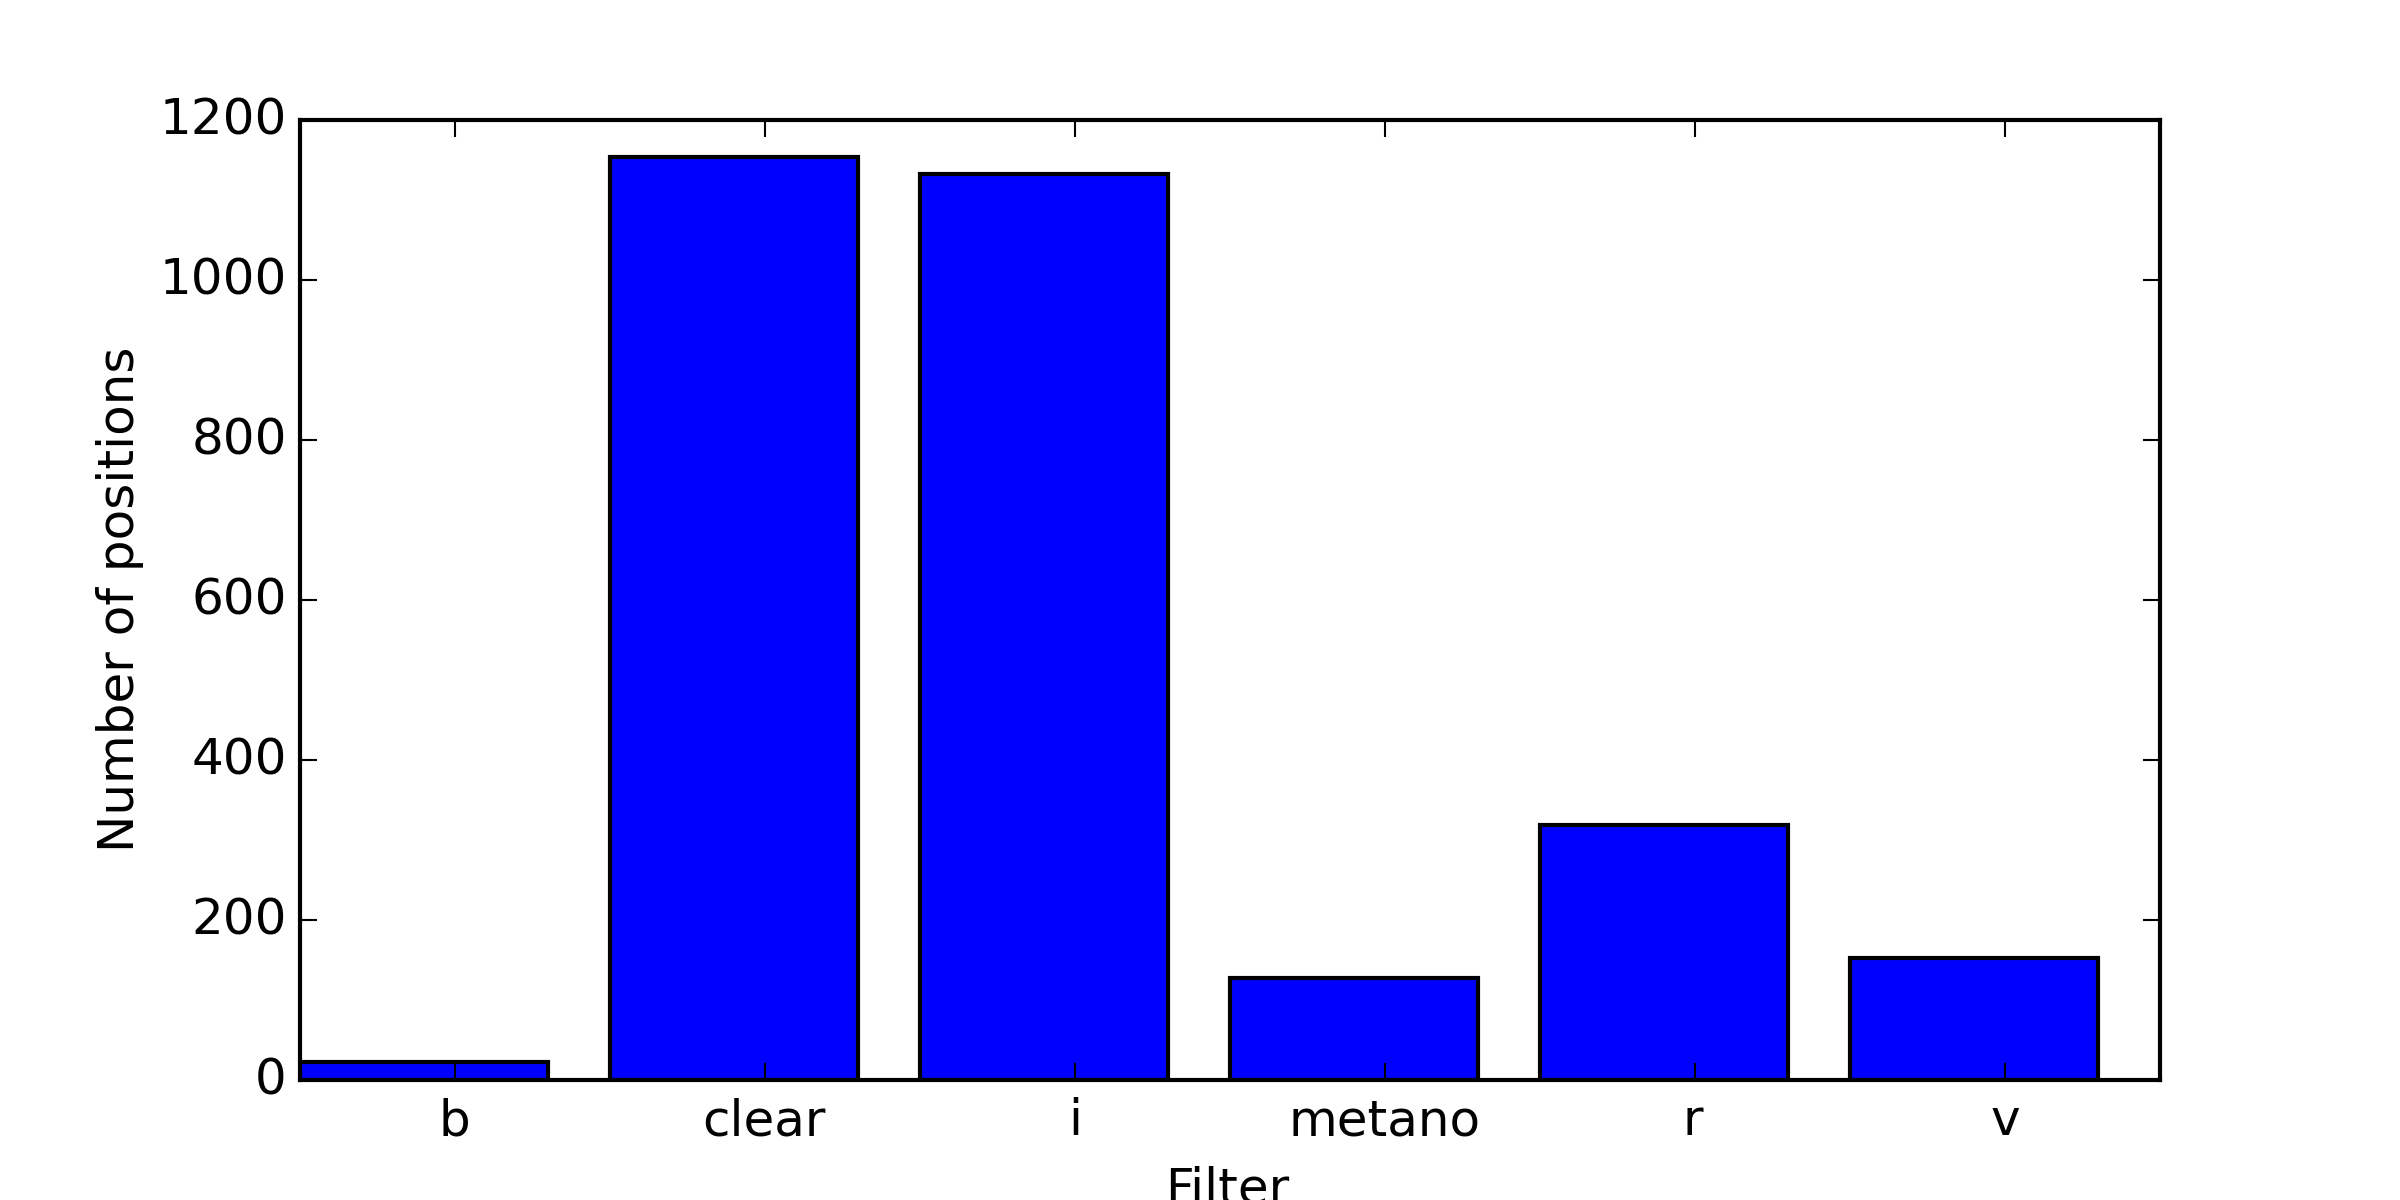
\includegraphics[width=16.0cm]{filtro_IAG.png} 
\caption{Distribution of positions by filter for the \BC telescope.}
\label{Fig:filtro-IAG}
\end{figure}

%\begin{longtable}{|c|c|c|c|c|c|c|}
%\caption{Same as in Table 2 for Neptune in the \BC telescope.}\\
%\hline
%Off-ra &  Off-de &   E-ra &   E-de & Nfr & Date & Ncat \\
%\hline
%\endfirsthead
%\multicolumn{7}{c}%
%{\tablename\ \thetable\ -- \textit{Continued from previous page}} \\
%\hline
%off-ra &  off-de &   E-ra &   E-de & Nfr & Date & Ncat \\
%\hline
%\endhead
%\hline \multicolumn{7}{r}{\textit{Continued on next page}} \\
%\endfoot
%\hline
%\endlastfoot
%-88.1 & -27.4 & 45.3 & 38.3 &  15 & 1995-09-17 00:20:52 &  12 \\
%84.6 & -37.8 & 57.0 & 33.2 &  37 & 2001-08-26 03:04:29 &  14 \\
%-128.1 & 160.8 & 25.6 & 33.1 &  20 & 2002-07-15 02:26:50 &  15 \\
%-43.4 & 194.3 & 22.6 & 22.4 &  18 & 2002-07-16 03:30:59 &  14 \\
%-56.4 & 205.5 & 21.2 & 19.1 &  24 & 2002-07-17 03:16:02 &  15 \\
%-185.5 & -155.8 & 49.9 & 46.2 &  17 & 2002-07-18 02:00:52 &  11 \\
%45.7 & -34.8 & 33.0 & 40.7 &  24 & 2003-07-22 05:21:32 &  16 \\
%-80.5 & 7.4 & 27.9 & 24.9 &  25 & 2003-07-23 03:42:29 &  18 \\
%-82.7 & -11.3 & 25.9 & 35.8 &  15 & 2003-07-24 02:27:29 &  18 \\
%-104.4 & 25.9 & 33.4 & 23.8 &  35 & 2003-07-25 03:25:27 &  14 \\
%-91.4 & -4.3 & 42.4 & 34.5 &  35 & 2003-07-26 04:14:22 &  15 \\
%-13.7 & -1.1 & 77.4 & 40.0 &  16 & 2003-07-27 07:07:07 &  14 \\
%-80.4 & 20.0 & 33.9 & 38.7 &  36 & 2003-07-28 04:24:57 &  16 \\
%85.9 & -63.9 & 75.2 & 11.3 &  20 & 2003-08-20 02:23:25 &  20 \\
%12.3 & 19.0 & 15.2 & 34.6 &   7 & 2003-10-14 23:10:27 &  29 \\
%3.2 & 7.7 & 32.2 & 17.8 &   6 & 2003-10-15 22:42:13 &  30 \\
%-11.8 & -54.8 & 58.6 & 59.4 &   5 & 2003-10-16 23:48:10 &  23 \\
%-3.2 & -69.0 & 67.1 & 44.0 &   4 & 2003-10-19 23:28:27 &  25 \\
%17.6 & -93.6 & 42.0 & 56.6 &  11 & 2004-08-05 05:30:15 &  13 \\
%63.6 & -144.2 & 77.4 & 51.9 &   9 & 2004-08-06 04:09:25 &  14 \\
%108.2 & -130.3 & 75.4 & 25.5 &  13 & 2004-08-07 03:14:48 &  19 \\
%22.8 & -88.1 & 63.5 & 69.0 &   8 & 2004-08-08 01:23:21 &  19 \\
%49.8 & -78.8 & 46.6 & 29.5 &  17 & 2004-08-20 02:42:31 &  24 \\
%-30.4 & -79.9 & 48.7 & 55.3 &  28 & 2004-08-21 03:12:05 &  21 \\
%-44.0 & -72.8 & 18.2 & 31.2 &  24 & 2004-08-22 01:17:29 &  20 \\
%-7.0 & -77.2 & 40.3 & 33.7 &  51 & 2004-08-23 03:12:09 &  17 \\
%-0.6 & -82.8 & 28.0 & 33.0 &  30 & 2004-08-24 03:24:43 &  17 \\
%104.7 & 13.1 & 52.9 & 75.7 &  12 & 2004-09-23 00:43:43 &  12 \\
%110.1 & 87.6 & 79.5 & 77.9 &  18 & 2004-09-24 01:04:29 &  14 \\
%150.9 & -1.4 & 64.3 & 43.4 &  19 & 2004-09-25 01:20:55 &  14 \\
%-0.3 & -87.3 & 19.8 & 37.3 & 111 & 2005-09-24 02:57:13 &  16 \\
%-26.8 & -79.8 & 38.7 & 35.2 &  38 & 2006-06-07 07:07:55 &  23 \\
%-111.0 & -102.2 & 79.9 & 63.3 & 107 & 2006-06-08 06:33:44 &  27 \\
%42.1 & -82.5 & 18.8 & 48.6 &  28 & 2006-07-04 05:13:37 &  12 \\
%-90.8 & -23.1 & 38.9 & 39.7 &  27 & 2006-08-30 00:57:08 &  16 \\
%52.8 & -37.7 & 33.1 & 36.0 &  18 & 2006-08-31 02:31:20 &  19 \\
%53.5 & -45.3 & 24.0 & 38.0 &  21 & 2006-09-01 02:34:07 &  19 \\
%45.0 & -54.5 & 21.6 & 25.4 &  21 & 2006-09-04 02:39:49 &  17 \\
%54.9 & -48.1 & 35.2 & 25.5 &  16 & 2006-09-05 03:07:34 &  13 \\
%68.5 & -42.3 & 26.8 & 34.4 &  41 & 2006-09-06 02:30:36 &  12 \\
%208.7 & -56.9 & 64.4 & 48.4 &  40 & 2006-09-09 04:00:58 &  18 \\
%277.6 & -59.8 & 64.3 & 79.7 &  34 & 2006-09-11 04:28:42 &  17 \\
%396.6 & -107.9 & 77.0 & 76.4 &  20 & 2006-09-12 05:10:52 &  15 \\
%146.4 & -39.4 & 25.2 & 46.1 &  38 & 2006-09-20 02:19:30 &  18 \\
%67.1 & -36.8 & 20.8 & 23.7 &  38 & 2006-09-22 01:39:33 &  20 \\
%93.8 & -38.2 & 15.0 & 23.8 &  18 & 2006-09-25 01:32:35 &  17 \\
%8.3 & -32.4 & 61.0 & 77.7 &  12 & 2006-10-20 23:04:59 &   9 \\
%-13.6 & -40.7 & 38.5 & 29.4 &  20 & 2006-10-21 22:15:23 &  13 \\
%70.4 & -42.4 & 50.0 & 41.6 &  23 & 2006-10-22 23:17:17 &  12 \\
%3.1 & -18.4 & 49.9 & 26.0 &  12 & 2006-10-25 22:21:13 &  31 \\
%198.8 & -115.7 & 49.6 & 36.8 &  44 & 2007-09-17 03:26:02 &  19 \\
%13.1 & -155.5 & 12.7 & 16.3 &  27 & 2008-09-20 03:37:18 &  25 \\
%8.5 & -62.2 & 22.7 & 26.5 &  22 & 2009-07-18 03:58:13 &  18 \\
%34.2 & 78.1 & 26.6 & 40.4 &  22 & 2009-07-20 06:04:51 &  14 \\
%-51.7 & -75.1 & 23.6 & 30.6 &  13 & 2009-07-21 07:07:08 &  13 \\
%20.5 & 11.1 & 54.8 & 68.0 &  11 & 2009-07-22 05:40:51 &  13 \\
%153.4 & -253.8 & 16.3 & 46.9 &  30 & 2010-07-04 08:22:47 &  15 \\
%151.8 & -192.4 & 68.7 & 75.9 &  10 & 2010-07-05 07:14:23 &  20 \\
%-35.4 & -148.7 & 60.8 & 21.0 &  74 & 2010-09-05 02:30:35 &  12 \\
%-12.7 & -26.9 & 25.3 & 36.5 &  18 & 2011-05-24 08:13:36 &   8 \\
%57.5 & -312.8 & 78.7 & 72.4 &  15 & 2011-08-19 04:17:47 &  10 \\
%73.2 & -162.4 & 33.6 & 10.8 &  26 & 2011-09-03 05:31:28 &  13 \\
%35.2 & -122.4 & 28.2 & 21.4 &  51 & 2011-09-04 03:54:40 &  18 \\
%-290.8 & -121.0 & 79.4 & 22.3 &  48 & 2011-09-05 02:57:52 &  19 \\
%131.3 & -97.9 & 47.3 & 33.3 &  23 & 2011-09-10 05:57:17 &  10 \\
%14.0 & -18.6 & 13.2 & 14.6 &  72 & 2011-09-23 01:09:04 &  16 \\
%58.8 & -45.3 & 19.2 & 24.6 & 131 & 2011-09-26 02:41:36 &  17 \\
%35.9 & -5.4 & 12.8 & 13.9 &  42 & 2011-09-27 01:34:13 &  19 \\
%31.5 & -114.5 & 16.7 & 20.3 &  23 & 2011-10-24 23:19:04 &  21 \\
%43.5 & -134.9 & 35.3 & 11.8 &  30 & 2011-10-26 23:40:14 &  19 \\
%-142.4 & -3.4 & 14.7 & 41.8 &  18 & 2012-07-22 04:06:19 &   7 \\
%-116.4 & -94.6 & 60.6 & 53.6 &  28 & 2012-08-24 05:00:16 &  14 \\
%21.3 & -125.5 & 36.7 & 15.4 &  19 & 2012-09-15 02:35:47 &  11 \\
%-54.8 & -107.4 & 22.3 & 22.6 &  26 & 2012-09-15 23:32:44 &  10 \\
%-50.8 & -128.8 & 28.2 & 31.7 &  25 & 2012-09-17 00:57:30 &  12 \\
%-30.6 & -127.9 & 26.8 & 22.5 &  24 & 2012-09-18 01:41:33 &  13 \\
%-39.4 & -97.6 & 35.4 & 31.7 &  25 & 2012-09-19 01:11:55 &  15 \\
%54.9 & -153.3 & 47.4 & 79.0 &  81 & 2012-10-19 01:55:57 &   8 \\
%3.3 & -17.8 & 48.3 & 31.6 &  30 & 2013-05-05 08:00:52 &  15 \\
%16.3 & 20.8 & 14.7 & 21.3 &  17 & 2013-05-09 08:28:00 &  17 \\
%14.6 & 11.6 & 58.7 & 16.2 &  19 & 2013-05-10 08:22:58 &  16 \\
%3.5 & 27.4 & 26.4 & 25.6 &  39 & 2013-07-12 06:56:33 &  18 \\
%18.3 & -12.7 & 36.4 & 41.6 &  39 & 2013-07-13 06:13:34 &  18 \\
%0.0 & 8.5 & 22.7 & 19.2 &  37 & 2013-07-15 07:18:49 &  18 \\
%107.4 & -65.1 & 35.4 & 25.7 &   9 & 2013-09-06 04:24:17 &   8 \\
%2.9 & -73.1 & 18.8 & 20.3 &  42 & 2013-09-07 03:09:30 &   7 \\
%41.2 & -77.2 & 24.3 & 36.3 &  21 & 2013-09-10 03:29:31 &  10 \\
%-170.5 & -8.3 & 76.1 & 65.7 &  20 & 2014-07-30 04:05:46 &   5 \\
%24.8 & -8.4 & 30.0 & 38.2 &  38 & 2014-07-31 02:40:38 &   5 \\
%-109.9 & -114.0 & 28.8 & 22.8 &  49 & 2014-09-13 03:07:20 &  20 \\
%33.0 & 40.3 & 19.8 & 32.7 &  34 & 2015-09-25 04:19:27 &  15 \\
%\hline
%\end{longtable}
%
%\begin{longtable}{|c|c|c|c|c|c|c|}
%\caption{Same as in Table 2 for Triton in the \BC telescope.}\\
%\hline
%Off-ra &  Off-de &   E-ra &   E-de & Nfr & Date & Ncat \\
%\hline
%\endfirsthead
%\multicolumn{7}{c}%
%{\tablename\ \thetable\ -- \textit{Continued from previous page}} \\
%\hline
%off-ra &  off-de &   E-ra &   E-de & Nfr & Date & Ncat \\
%\hline
%\endhead
%\hline \multicolumn{7}{r}{\textit{Continued on next page}} \\
%\endfoot
%\hline
%\endlastfoot
%-93.3 & -58.1 & 39.7 & 22.2 &  21 & 1995-09-17 00:26:00 &  13 \\
%-14.3 & -65.1 & 27.7 & 40.4 &  19 & 2001-08-26 02:53:22 &  14 \\
%11.7 & -26.7 & 27.5 & 16.2 &  36 & 2002-07-15 05:00:25 &  17 \\
%-2.4 & -25.0 & 19.3 & 24.2 &  12 & 2002-07-16 03:30:20 &  15 \\
%-7.1 & -43.5 & 20.0 & 20.8 &  17 & 2002-07-17 03:14:54 &  15 \\
%19.9 & -68.8 & 38.6 & 25.6 &  19 & 2002-07-18 03:12:12 &  14 \\
%-11.6 & -0.9 & 38.2 & 27.7 &  22 & 2003-07-22 06:16:18 &  17 \\
%-45.0 & -10.6 & 51.7 & 31.4 &  33 & 2003-07-23 03:16:44 &  16 \\
%-71.5 & 2.9 & 36.2 & 32.5 &  15 & 2003-07-24 02:27:01 &  18 \\
%-84.9 & 12.6 & 36.1 & 24.4 &  26 & 2003-07-25 03:42:51 &  15 \\
%-70.7 & 32.0 & 77.4 & 33.8 &  32 & 2003-07-26 03:39:33 &  18 \\
%-40.2 & 35.3 & 76.8 & 68.7 &  26 & 2003-07-27 07:08:17 &  13 \\
%-76.3 & 26.0 & 22.5 & 33.3 &  28 & 2003-07-28 04:26:58 &  18 \\
%59.5 & -3.1 & 45.8 & 22.1 &  33 & 2003-08-20 03:29:36 &  21 \\
%-5.5 & 15.4 & 15.8 & 16.1 &  11 & 2003-10-14 23:31:14 &  33 \\
%-21.9 & -2.9 & 39.1 & 79.8 &  18 & 2003-10-15 23:12:31 &  33 \\
%-18.5 & -14.6 & 68.0 & 38.4 &   8 & 2003-10-17 00:27:54 &  25 \\
%10.3 & 36.4 & 29.5 & 78.2 &   8 & 2003-10-17 23:59:42 &  28 \\
%-7.2 & -45.2 & 41.4 & 36.1 &  12 & 2003-10-19 23:39:48 &  31 \\
%-11.1 & -111.8 & 26.3 & 17.4 &  17 & 2004-08-05 05:23:17 &  16 \\
%98.5 & -92.8 & 9.7 & 20.5 &  15 & 2004-08-06 03:48:57 &  18 \\
%45.9 & -105.5 & 14.8 & 12.8 &  15 & 2004-08-07 03:00:16 &  21 \\
%21.9 & -95.5 & 38.3 & 46.0 &   8 & 2004-08-08 01:23:21 &  19 \\
%-6.5 & -36.3 & 26.9 & 19.9 &  15 & 2004-08-20 03:13:55 &  24 \\
%-9.6 & -45.8 & 38.6 & 40.7 &  23 & 2004-08-21 03:06:38 &  21 \\
%-3.4 & -64.3 & 17.8 & 27.5 &  20 & 2004-08-22 01:20:47 &  21 \\
%-8.5 & -37.1 & 20.1 & 23.1 &  27 & 2004-08-23 02:57:26 &  18 \\
%-6.5 & -35.9 & 21.2 & 34.3 &  22 & 2004-08-24 03:12:56 &  17 \\
%95.9 & -3.9 & 76.2 & 72.2 &   7 & 2004-09-23 00:45:10 &  13 \\
%66.5 & 119.6 & 64.4 & 75.7 &  22 & 2004-09-24 01:38:04 &  14 \\
%50.6 & 93.8 & 67.2 & 50.3 &  29 & 2004-09-25 02:06:53 &  14 \\
%-3.8 & 219.0 & 25.5 & 22.9 &   4 & 2004-10-08 23:29:18 &  20 \\
%-18.6 & -85.6 & 24.5 & 29.3 & 107 & 2005-09-24 02:50:15 &  16 \\
%8.9 & -48.2 & 23.0 & 29.4 &  38 & 2006-06-07 07:03:05 &  24 \\
%-5.9 & -55.8 & 42.7 & 38.9 &  96 & 2006-06-08 06:48:11 &  27 \\
%-11.6 & -67.2 & 24.1 & 18.7 &  19 & 2006-07-02 06:36:56 &  17 \\
%33.0 & -67.3 & 31.7 & 46.8 &  32 & 2006-07-04 05:12:04 &  12 \\
%80.5 & -57.3 & 56.3 & 38.7 &  20 & 2006-08-30 00:56:45 &  17 \\
%24.9 & 12.0 & 13.1 & 35.9 &  20 & 2006-09-01 02:35:19 &  20 \\
%-8.6 & 1.1 & 21.7 & 13.9 &  17 & 2006-09-04 02:40:26 &  17 \\
%21.0 & -4.9 & 14.4 & 35.6 &  12 & 2006-09-05 03:06:40 &  14 \\
%-7.1 & -15.6 & 26.9 & 28.7 &  39 & 2006-09-06 02:31:52 &  13 \\
%26.6 & 36.1 & 61.8 & 46.7 &  34 & 2006-09-09 04:01:33 &  18 \\
%-8.9 & 47.6 & 56.5 & 79.6 &  31 & 2006-09-11 04:28:38 &  16 \\
%20.4 & 1.8 & 78.8 & 78.2 &  20 & 2006-09-12 05:10:45 &  15 \\
%35.4 & 9.5 & 30.2 & 59.3 &  44 & 2006-09-20 02:18:01 &  17 \\
%20.4 & 1.8 & 12.1 & 29.1 &  35 & 2006-09-22 01:40:29 &  20 \\
%24.6 & -9.7 & 10.5 & 26.0 &  18 & 2006-09-25 01:31:52 &  19 \\
%-0.2 & 26.3 & 59.9 & 78.8 &  12 & 2006-10-20 23:05:50 &   9 \\
%-11.9 & 16.0 & 23.4 & 47.1 &  20 & 2006-10-21 22:16:11 &  14 \\
%-0.0 & -48.8 & 46.0 & 44.3 &  22 & 2006-10-22 23:16:45 &  12 \\
%0.6 & 29.3 & 19.5 & 35.1 &  14 & 2006-10-25 22:14:59 &  30 \\
%15.5 & -29.0 & 50.0 & 31.9 &  34 & 2007-09-17 03:21:45 &  18 \\
%-27.4 & -92.6 & 6.2 & 12.2 &  23 & 2008-09-20 03:38:08 &  24 \\
%-44.9 & -23.3 & 15.3 & 22.5 &  26 & 2009-07-18 03:59:51 &  19 \\
%-43.7 & 83.3 & 17.7 & 39.2 &  24 & 2009-07-20 06:04:37 &  15 \\
%-24.3 & -24.6 & 36.9 & 34.9 &  16 & 2009-07-21 07:03:50 &  14 \\
%8.8 & 62.5 & 27.6 & 79.6 &  13 & 2009-07-22 05:32:58 &  14 \\
%108.9 & -218.5 & 25.7 & 43.3 &  26 & 2010-07-04 08:23:03 &  15 \\
%76.2 & -28.4 & 23.1 & 7.9 &  17 & 2010-07-05 07:16:59 &  20 \\
%24.9 & -56.1 & 5.5 & 12.3 &  41 & 2010-09-05 02:29:34 &  12 \\
%-50.3 & 2.4 & 29.9 & 25.7 &   9 & 2011-05-24 08:13:00 &   8 \\
%-28.4 & -12.9 & 23.5 & 21.6 &  29 & 2011-08-19 04:10:39 &  10 \\
%81.2 & -57.1 & 25.5 & 16.6 &  28 & 2011-09-03 05:33:52 &  13 \\
%80.3 & -6.5 & 18.1 & 23.4 &  60 & 2011-09-04 03:38:42 &  19 \\
%58.4 & -27.5 & 6.3 & 6.0 &  33 & 2011-09-05 02:47:44 &  19 \\
%64.0 & -24.4 & 48.0 & 36.6 &  24 & 2011-09-10 05:57:16 &  10 \\
%31.7 & 7.9 & 12.2 & 10.6 &  87 & 2011-09-23 01:09:14 &  16 \\
%41.3 & 16.9 & 10.6 & 29.2 & 154 & 2011-09-26 02:52:52 &  17 \\
%52.6 & 56.3 & 9.9 & 13.5 &  47 & 2011-09-27 01:34:30 &  19 \\
%76.0 & -34.4 & 11.9 & 17.2 &  42 & 2011-10-24 23:39:03 &  21 \\
%63.4 & -47.3 & 11.5 & 9.8 &  45 & 2011-10-26 23:48:39 &  19 \\
%-133.3 & -6.4 & 41.4 & 53.8 &  25 & 2012-07-22 04:06:34 &   7 \\
%-64.3 & -45.3 & 48.4 & 48.2 &  27 & 2012-08-24 05:00:16 &  14 \\
%34.4 & -76.0 & 42.0 & 23.0 &  25 & 2012-09-15 02:35:48 &  11 \\
%4.4 & -47.2 & 27.4 & 13.6 &  23 & 2012-09-15 23:32:26 &  10 \\
%-19.7 & -61.4 & 30.8 & 21.9 &  23 & 2012-09-17 00:57:30 &  12 \\
%3.9 & -57.0 & 25.4 & 21.3 &  27 & 2012-09-18 01:41:38 &  13 \\
%-6.4 & -51.5 & 36.4 & 31.0 &  28 & 2012-09-19 01:11:45 &  15 \\
%21.7 & -48.2 & 38.8 & 79.6 &  68 & 2012-10-19 01:56:38 &   8 \\
%16.3 & 7.4 & 46.8 & 38.6 &  30 & 2013-05-05 08:00:35 &  16 \\
%15.4 & 11.8 & 9.4 & 17.9 &  18 & 2013-05-09 08:27:37 &  17 \\
%1.1 & 23.7 & 7.6 & 7.5 &  15 & 2013-05-10 08:22:39 &  16 \\
%20.9 & 24.9 & 20.2 & 25.6 &  33 & 2013-07-12 06:56:06 &  18 \\
%8.5 & 25.8 & 26.0 & 30.3 &  31 & 2013-07-13 06:13:33 &  18 \\
%32.8 & 36.1 & 11.4 & 10.0 &  36 & 2013-07-15 07:19:03 &  18 \\
%0.9 & -7.5 & 27.7 & 51.5 &  10 & 2013-09-06 04:24:20 &   8 \\
%8.8 & -56.1 & 19.6 & 15.7 &  38 & 2013-09-07 03:08:47 &   7 \\
%10.3 & -24.2 & 43.2 & 29.1 &  21 & 2013-09-10 03:30:03 &  10 \\
%-92.9 & -53.2 & 25.3 & 46.8 &  15 & 2014-07-30 04:05:39 &   5 \\
%10.4 & -2.0 & 26.5 & 35.8 &  37 & 2014-07-31 02:40:55 &   5 \\
%-61.4 & -99.4 & 20.1 & 20.9 &  50 & 2014-09-13 03:06:59 &  20 \\
%22.3 & 17.5 & 16.5 & 18.8 &  32 & 2015-09-25 04:19:38 &  15 \\
%\hline
%\end{longtable}
 
 
%\section*{Zeiss}


\begin{figure}
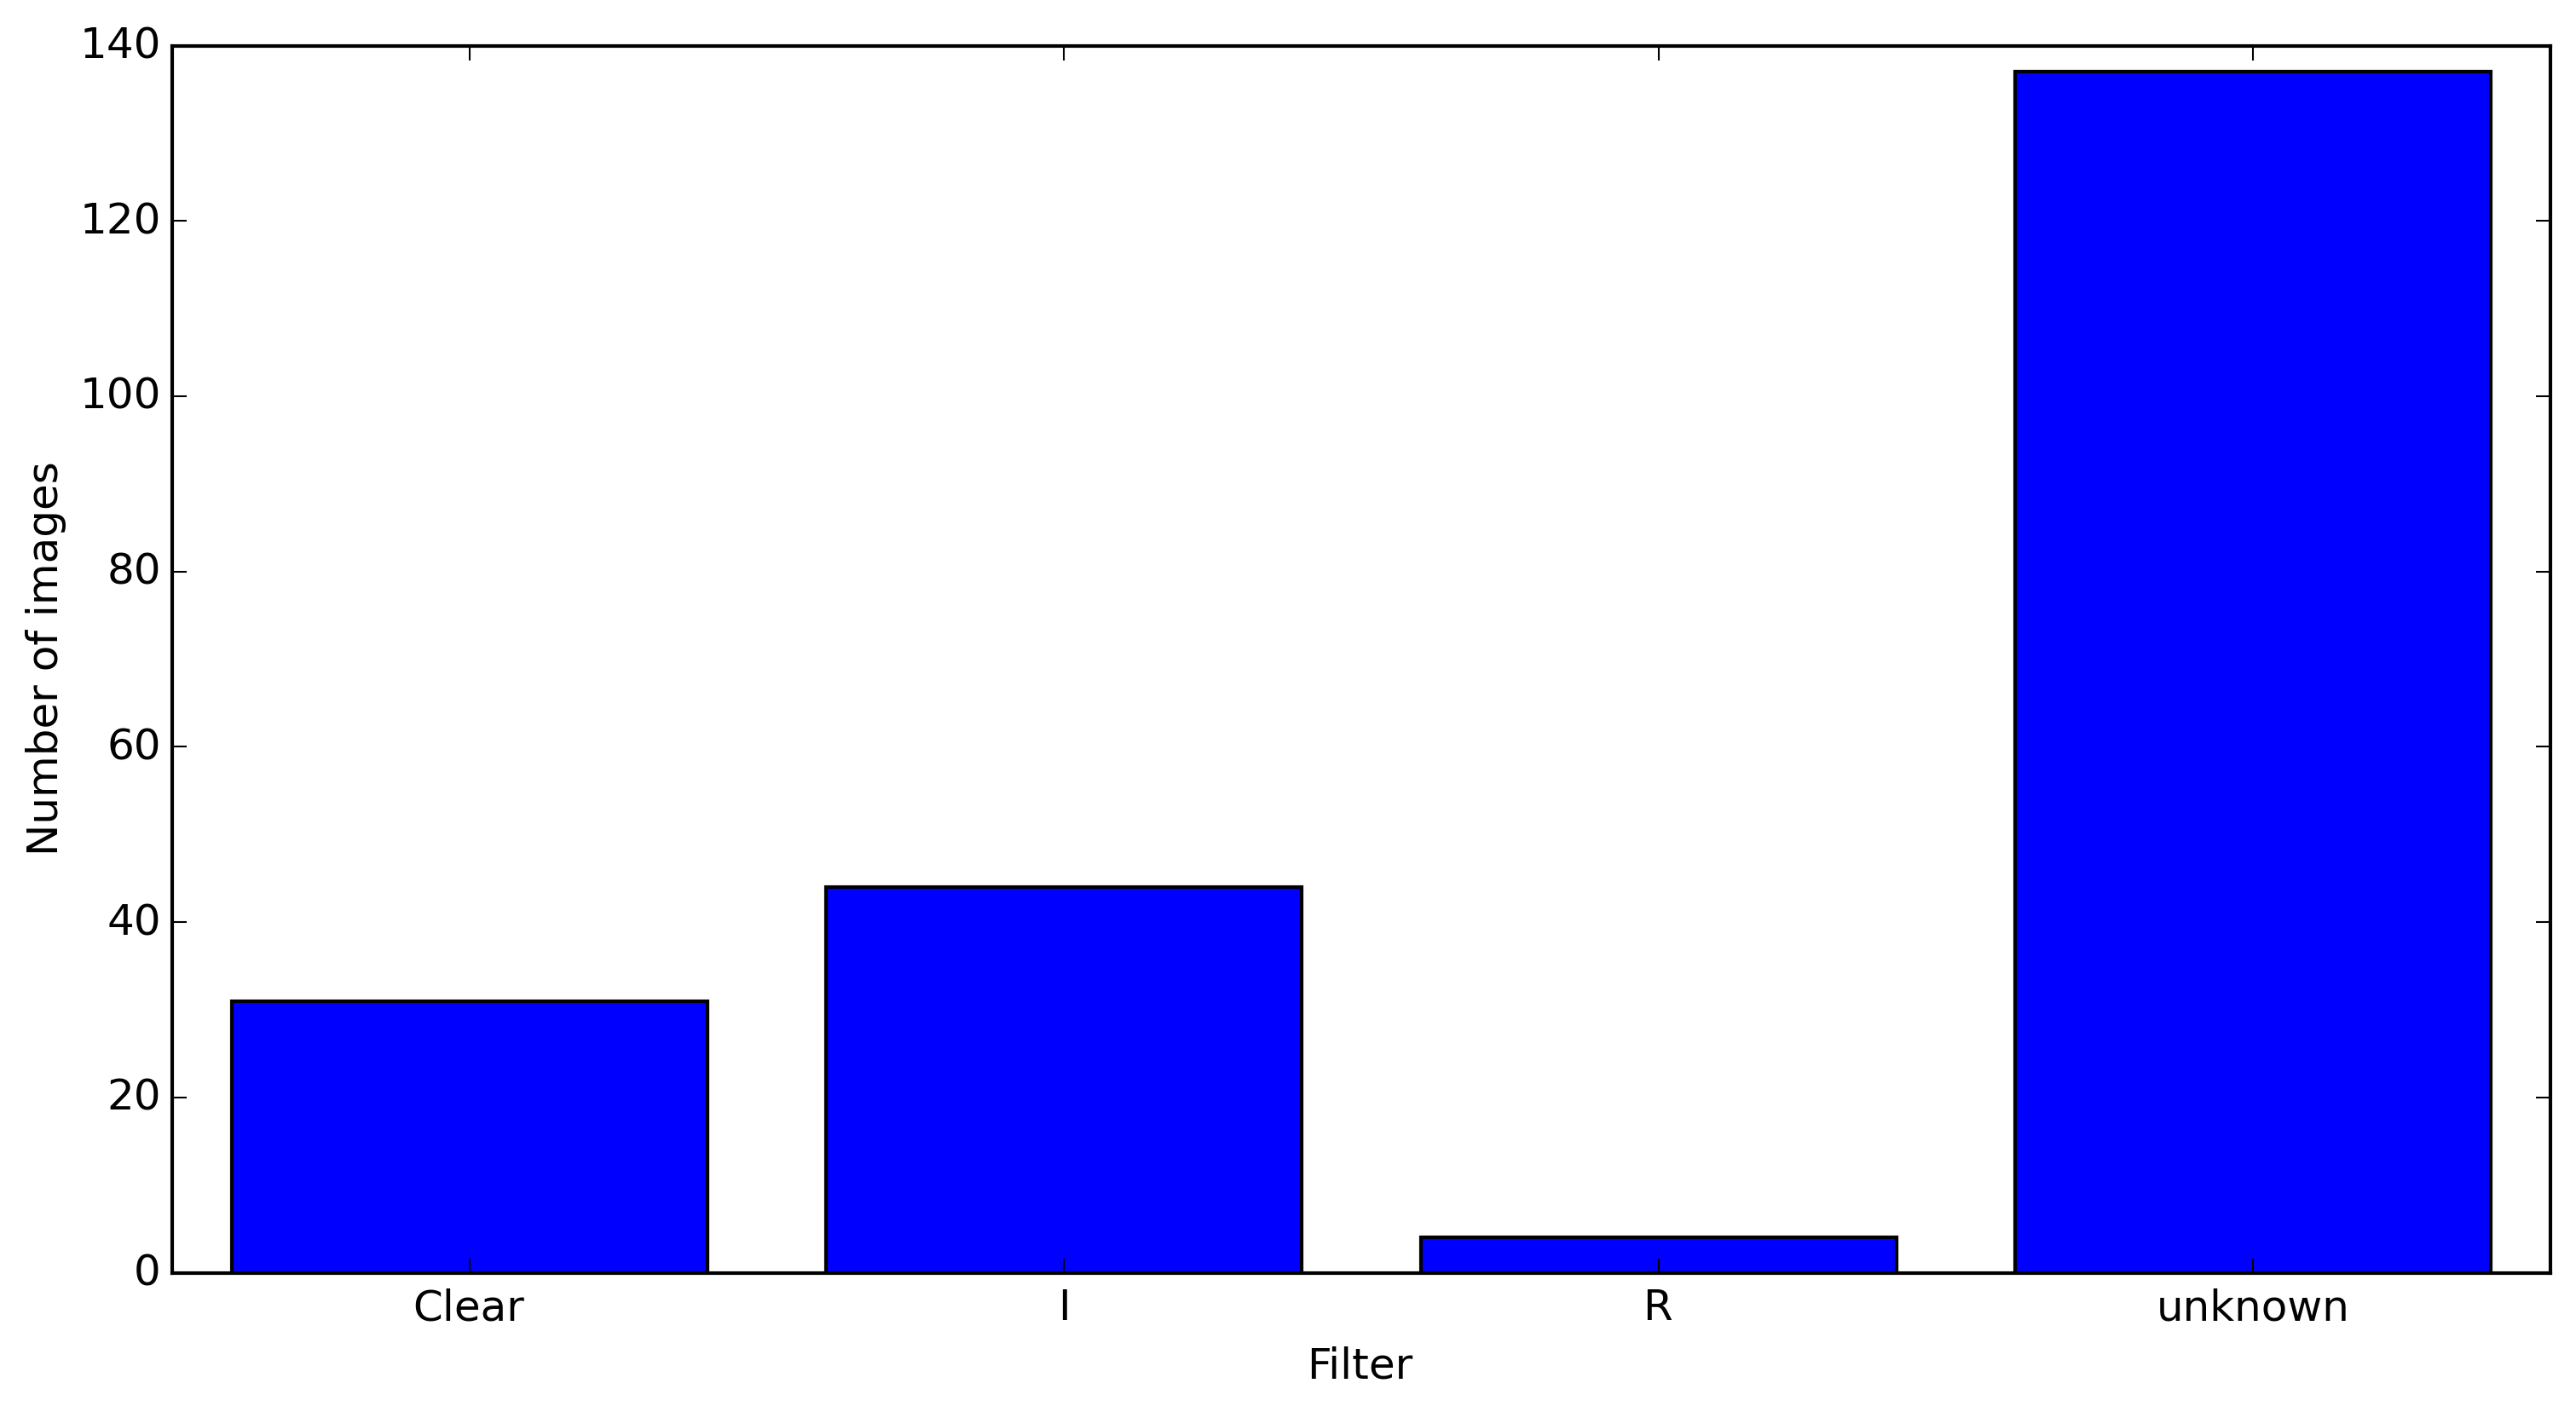
\includegraphics[width=16.0cm]{filtro_ZEI.png} 
\caption{Distribution of positions by filter for the Zeiss telescope.}
\label{Fig:filtro-ZEI}
\end{figure}
 
%\begin{longtable}{|c|c|c|c|c|c|c|}
%\caption{Same as in Table 2 for Neptune in the Zeiss telescope.}\\
%\hline
%Off-ra &  Off-de &   E-ra &   E-de & Nfr & Date & Ncat \\
%\hline
%\endfirsthead
%\multicolumn{7}{c}%
%{\tablename\ \thetable\ -- \textit{Continued from previous page}} \\
%\hline
%off-ra &  off-de &   E-ra &   E-de & Nfr & Date & Ncat \\
%\hline
%\endhead
%\hline \multicolumn{7}{r}{\textit{Continued on next page}} \\
%\endfoot
%\hline
%\endlastfoot
%-139.1 & -110.3 & 37.9 & 32.6 &  31 & 1996-07-17 00:52:38 &   9 \\
%-51.4 & -41.4 & 36.5 & 45.8 &  46 & 1996-07-18 01:57:03 &   8 \\
%31.9 & -85.1 & 32.6 & 29.9 &  48 & 1996-07-24 03:24:16 &  12 \\
%24.8 & -30.3 & 48.5 & 46.3 &  33 & 1996-07-30 01:42:55 &   7 \\
%-57.5 & -61.2 & 52.4 & 56.7 &   6 & 2008-05-15 04:57:18 &   7 \\
%35.1 & -54.0 & 16.3 & 16.5 &   8 & 2009-09-04 03:46:23 &  12 \\
%1.4 & -54.4 & 22.3 & 30.4 &  10 & 2009-09-05 01:16:48 &  15 \\
%169.5 & -194.4 & 7.9 & 11.9 &  66 & 2010-08-18 05:09:23 &  22 \\
%\hline
%\end{longtable}
%
%\begin{longtable}{|c|c|c|c|c|c|c|}
%\caption{Same as in Table 2 for Triton in the Zeiss telescope.}\\
%\hline
%Off-ra &  Off-de &   E-ra &   E-de & Nfr & Date & Ncat \\
%\hline
%\endfirsthead
%\multicolumn{7}{c}%
%{\tablename\ \thetable\ -- \textit{Continued from previous page}} \\
%\hline
%off-ra &  off-de &   E-ra &   E-de & Nfr & Date & Ncat \\
%\hline
%\endhead
%\hline \multicolumn{7}{r}{\textit{Continued on next page}} \\
%\endfoot
%\hline
%\endlastfoot
%8.4 & -9.1 & 19.5 & 48.0 &  40 & 1996-07-17 00:57:09 &  10 \\
%26.8 & 22.8 & 32.6 & 45.2 &  50 & 1996-07-18 01:59:54 &   8 \\
%33.3 & -11.1 & 11.5 & 29.3 &  36 & 1996-07-24 03:22:42 &  13 \\
%22.9 & -17.1 & 38.1 & 40.7 &  30 & 1996-07-30 01:43:06 &   7 \\
%2.5 & -48.0 & 42.7 & 71.9 &   4 & 2008-05-15 04:48:52 &   8 \\
%-12.2 & 6.9 & 33.4 & 33.1 &  10 & 2009-09-04 03:46:53 &  11 \\
%-13.7 & 2.9 & 31.9 & 26.3 &  10 & 2009-09-05 01:16:48 &  15 \\
%28.1 & -36.6 & 12.0 & 15.2 &  46 & 2010-05-29 08:34:42 &  23 \\
%105.0 & -104.6 & 7.0 & 22.9 & 120 & 2010-08-18 05:04:06 &  22 \\
%\hline
%\end{longtable}

\begin{longtable}{|l|c|c|c|c|}
\caption{Table of erros of the reduction. Gaussian error stands for the error in X and Y of the bidimensional Gaussian used to fit the PSF. Mean offset errors is the average dispersion of the positions of each night.}\\
\hline
Telescope/Satellite &  \multicolumn{2}{|c|}{Gaussian error} &   \multicolumn{2}{|c|}{Mean offet errors} \\
%\hline
 &  X (mas) & Y (mas) & RA (mas) & DEC (mas) \\
\hline
\endfirsthead
\multicolumn{5}{c}%
{\tablename\ \thetable\ -- \textit{Continued from previous page}} \\
\hline
Telescope/Satellite &  X & Y & RA & DEC \\
\hline
\endhead
\hline \multicolumn{5}{r}{\textit{Continued on next page}} \\
\endfoot
\hline
\endlastfoot
160/Neptune & 8 & 8 & 42 & 37 \\
160/Triton & 14 & 14 & 28 & 29 \\
IAG/Neptune & 9 & 9 & 36 & 38 \\
IAG/Triton & 20 & 20 & 34 & 37 \\
Zeiss/Neptune & 9 & 9 & 28 & 32 \\
Zeiss/Triton & 27 & 27 & 28 & 35 \\
\hline
\end{longtable}

%\bibliography{Referencias}
%\bibliographystyle{apalike}


\end{document}
